% Version 3.1 December 2024
% HPR Probabilistic Surrogate Paper
% English text (compilable with pdflatex); Chinese translation in comments (%CN:)

\documentclass[pdflatex,sn-mathphys-num]{sn-jnl}

%%%% Standard Packages
\usepackage{graphicx}
\usepackage{multirow}
\usepackage{amsmath,amssymb,amsfonts}
\usepackage{amsthm}
\usepackage{mathrsfs}
\usepackage[title]{appendix}
\usepackage{xcolor}
\usepackage{textcomp}
\usepackage{manyfoot}
\usepackage{booktabs}
\usepackage{algorithm}
\usepackage{algorithmicx}
\usepackage{algpseudocode}
\usepackage{listings}
\usepackage{siunitx}      % for \SI, \num
\usepackage{bm}           % for \bm (bold math)
\usepackage{hyperref}

\theoremstyle{thmstyleone}
\newtheorem{theorem}{Theorem}
\newtheorem{proposition}[theorem]{Proposition}
\theoremstyle{thmstyletwo}
\newtheorem{example}{Example}
\newtheorem{remark}{Remark}
\theoremstyle{thmstylethree}
\newtheorem{definition}{Definition}

\raggedbottom % chktex 1

% ── Figure path ─────────────────────────────────────────────────────────────
% Figures live in figures/draft/ relative to the project root.
% When compiling from sn-article-template/, use:
\graphicspath{{../figures/draft/}}

\begin{document}

%CN: 题目：概率神经代理模型在耦合多物理场系统不确定性–风险分析中的应用：以热管冷却反应堆为例
\title[HPR Probabilistic Surrogate]{%
  Probabilistic neural surrogates for uncertainty-to-risk analysis
  in coupled multi-physics systems: application to a heat-pipe-cooled reactor}

\author*[1]{\fnm{First} \sur{Author}}\email{author@institution.edu}
\author[1]{\fnm{Second} \sur{Author}}
\author[1]{\fnm{Third} \sur{Author}}

\affil*[1]{\orgdiv{Department of Nuclear Engineering},
           \orgname{Institution},
           \orgaddress{\city{City}, \country{Country}}}

% -----------------------------------------------------------------------
%  Abstract
% -----------------------------------------------------------------------
%CN: 摘要
%CN: 本文针对热管冷却反应堆（HPR）耦合热-力分析开发了概率代理模型，能够以极低计算成本
%CN: 完成端到端的不确定性–风险定量分析。代理模型为异方差多层感知机（HeteroMLP），基于
%CN: 约2900次OpenMC–FEniCS耦合仿真数据训练。含物理约束的正则化变体（Level 2）通过嵌入
%CN: 单调性约束，在测试集上达到负对数似然0.305，应力R²=0.929（均方根误差7.9 MPa）。
%CN: 前向传播20000个先验蒙特卡洛样本揭示：耦合稳态应力均值较解耦预测低39 MPa（20%），
%CN: 标准差降低47%；keff不确定性压缩183倍；超过131 MPa设计阈值的概率为0.847。
%CN: Sobol分析识别SS316_k_ref为应力主控因素（S₁=0.529），alpha_base为keff主控因素
%CN: （S₁=0.481），表明两条独立物理传播路径。后验标定对全部10个极端应力案例（真实应力
%CN: ≥220 MPa）均使超阈概率收敛至1.0。代理模型推断速度比耦合高保真求解器快逾2300万倍。
\abstract{%
We develop a probabilistic surrogate framework for coupled thermo-mechanical
analysis of a heat-pipe-cooled reactor~(HPR), enabling end-to-end
uncertainty-to-risk quantification at a fraction of the cost of high-fidelity
simulation.
The surrogate is a heteroscedastic multilayer perceptron~(HeteroMLP) trained on
\num{2900} coupled OpenMC--FEniCS simulations, predicting distributions over 15
physics outputs from 8 material uncertainty inputs across two fidelity levels:
a~decoupled first-pass prediction and a~converged coupled steady-state.
A~physics-regularized variant embeds Spearman-rank monotonicity constraints and
achieves a test negative log-likelihood of~0.305, with coupled steady-state maximum global
stress~$R^2=0.929$ (RMSE~=~\SI{7.9}{MPa}).
Forward propagation of \num{20000} prior Monte~Carlo samples reveals that
multi-physics coupling substantially compresses uncertainty: the coupled stress
mean is \SI{39}{MPa} lower than the decoupled prediction (\SI{153}{MPa} vs.\ \SI{193}{MPa}),
with standard deviation reduced by~47\%; keff uncertainty collapses by~$183\times$.
The predicted probability of exceeding the \SI{131}{MPa} design threshold is
$0.847$ under the prior.
Sobol sensitivity analysis identifies SS316 thermal conductivity~(SS316$\_$k$\_$ref)
as the dominant stress driver ($S_1 = 0.529$) and thermal expansion
coefficient~(alpha$\_$base) as the dominant keff driver ($S_1 = 0.481$),
indicating independent physical pathways.
Posterior calibration over 20 benchmark cases demonstrates that, for all ten
extreme-stress scenarios with observed stress $\geq\SI{220}{MPa}$, the posterior
probability of exceeding \SI{131}{MPa} converges to~1.0.
The surrogate achieves a single-sample GPU latency of $\SI{1.7e-7}{s}$,
representing a speedup of more than $23\times10^{6}$ over the coupled solver.}

\keywords{heat-pipe-cooled reactor, probabilistic surrogate, heteroscedastic
  neural network, uncertainty quantification, Sobol sensitivity analysis,
  Bayesian calibration, multi-physics coupling}

\maketitle

% -----------------------------------------------------------------------
%  1. Introduction
% -----------------------------------------------------------------------
\section{Introduction}\label{sec:intro}

%CN: 引言
%CN: 热管冷却反应堆（HPR）作为一种新兴微型反应堆设计，其核心由紧密耦合的热管、燃料棒和
%CN: 单石结构组成，材料性能的不确定性通过复杂的热-力-中子耦合关系传播并放大为结构应力
%CN: 风险。精确的安全评估要求在材料不确定性的全空间上进行前向UQ分析和观测驱动的逆向标定，
%CN: 而每次耦合高保真仿真约需1小时，使暴力蒙特卡洛方法在实际工程中不可行。

Heat-pipe-cooled reactors~(HPRs) are an emerging class of compact microreactors
in which the core comprises tightly coupled heat pipes, fuel rods, and monolith
structures~\cite{ref:hpr_design}.
Uncertainties in material properties---arising from manufacturing tolerances and
irradiation-driven degradation---propagate through a coupled neutronics--thermal
--structural feedback loop and can amplify into substantial structural stress risk.
Prior high-fidelity analysis of the nominal MegaPower design reports peak monolith
stresses reaching \SI{169}{MPa} under normal operating conditions~\cite{ref:zhang2025energy},
which exceeds the yield strength of the SS316 stainless-steel monolith at reactor
operating temperatures (\SI{131}{MPa}); characterising how material-parameter
uncertainty translates into exceedance probability is therefore a~primary safety concern.
Quantifying this risk requires sampling over the full 8-dimensional material
parameter space, which is infeasible with repeated high-fidelity (HF) solver
evaluations: each coupled OpenMC--FEniCS run takes approximately one
hour~\cite{ref:openmc,ref:fenics}.

%CN: 现有方法的局限：高斯过程和多项式混沌展开在8维输入下遭遇维度诅咒；物理信息神经网络
%CN: 在耦合多物理场边界条件下难以构造精确残差。本文提出的HeteroMLP方法基于数据驱动，
%CN: 并通过物理正则化（单调性约束）提升泛化性，同时支持前向UQ、灵敏度分析和后验标定。

Existing surrogate approaches face complementary limitations.
Gaussian process~(GP) regression and polynomial chaos expansion~(PCE) become
computationally prohibitive as the input dimension grows, and require additional
regularity assumptions that may not hold across the full uncertainty
range~\cite{ref:gp_uq,ref:pce_uq}.
Physics-informed neural networks~(PINNs) are designed for problems where exact
governing equations can be expressed as residuals; the iterative coupling
boundary conditions in an HPR preclude this formulation~\cite{ref:pinn_review}.
Data-driven neural surrogates offer scalable inference but typically lack
uncertainty calibration and physical consistency guarantees.

%CN: 本文贡献：（1）异方差MLP预测15个输出的均值和方差；（2）Spearman秩单调性正则化
%CN: 提升OOD泛化；（3）完整的UQ流程：前向传播、Sobol灵敏度分析、MCMC后验标定；
%CN: （4）定量揭示iter1→iter2耦合对不确定性压缩的机制。

This work makes four contributions.
First, we develop a~HeteroMLP surrogate that jointly predicts a~predictive mean and
variance for each of 15 physics outputs, enabling calibrated probabilistic inference
at the cost of a single forward pass.
Second, we propose a~physics-regularized training objective that augments the
Gaussian negative log-likelihood~(NLL) with a~Spearman-rank monotonicity term
encoding known input--output relationships, and demonstrate substantially improved
out-of-distribution~(OOD) generalization.
Third, we present a~complete uncertainty-to-risk pipeline: forward Monte~Carlo
propagation, global Sobol sensitivity analysis with bootstrap confidence intervals,
and MCMC-based posterior calibration.
Fourth, we quantify---for the first time in this system---the degree to which
multi-physics coupling compresses material-parameter-driven uncertainty, revealing a
$183\times$ reduction in keff spread and a~47\% reduction in stress standard deviation
between the decoupled and coupled fidelity levels.

%CN: 本文结构：第2节介绍代理模型架构、训练目标和四条分析流程；第3节报告测试集精度、
%CN: 前向不确定性传播、灵敏度归因和后验标定结果；第4节讨论主要发现的物理含义与方法局限；
%CN: 第5节总结核心结论。
The remainder of the paper is organised as follows.
Section~\ref{sec:methods} details the surrogate architecture, training objectives,
and the four analysis pipelines.
Section~\ref{sec:results} reports test-set accuracy, forward uncertainty propagation,
sensitivity attribution, and posterior calibration results.
Section~\ref{sec:discussion} discusses physical and practical implications and
identifies limitations.
Section~\ref{sec:conclusion} summarises the principal findings.

% ── Fig 1 ─────────────────────────────────────────────────────────────────
%CN: 图1（v1）：从材料不确定性到风险定量的完整代理框架流程图（水平布局）。
%CN: 图1（v2）：垂直布局版本，展示从参数采样到代理推断再到分析流水线的完整路径。
\begin{figure}[ht]
  \centering
  % v1: horizontal pipeline layout — 4 stages left to right
  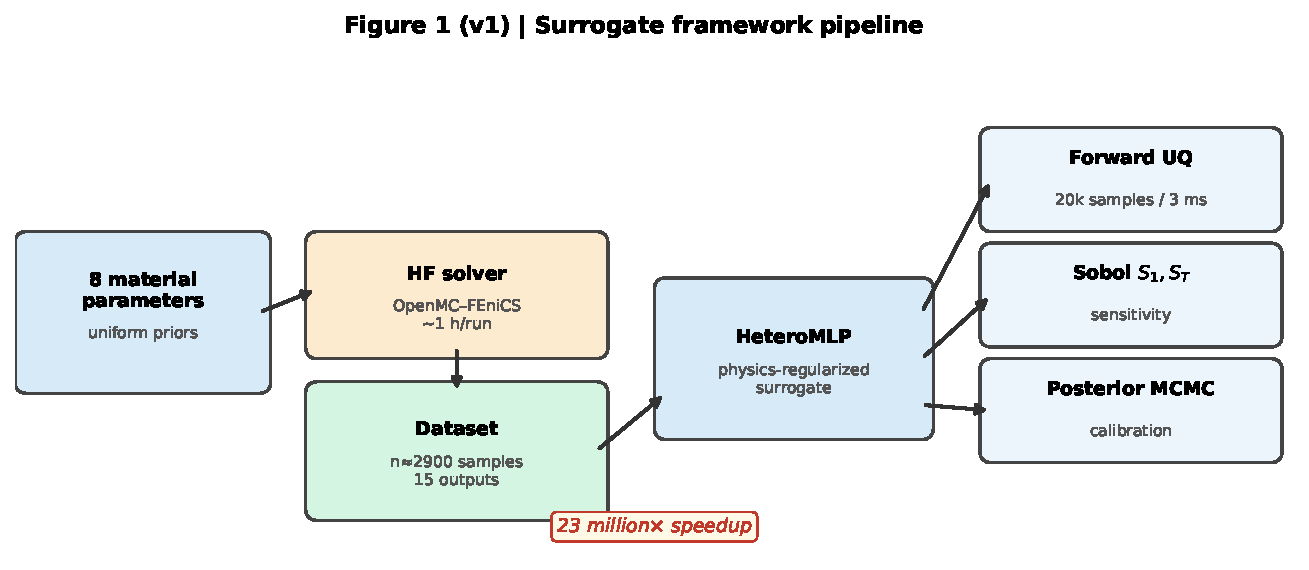
\includegraphics[width=\textwidth]{fig1_framework_v1}\\[8pt]
  % v2: vertical layout (choose one for final submission)
  % 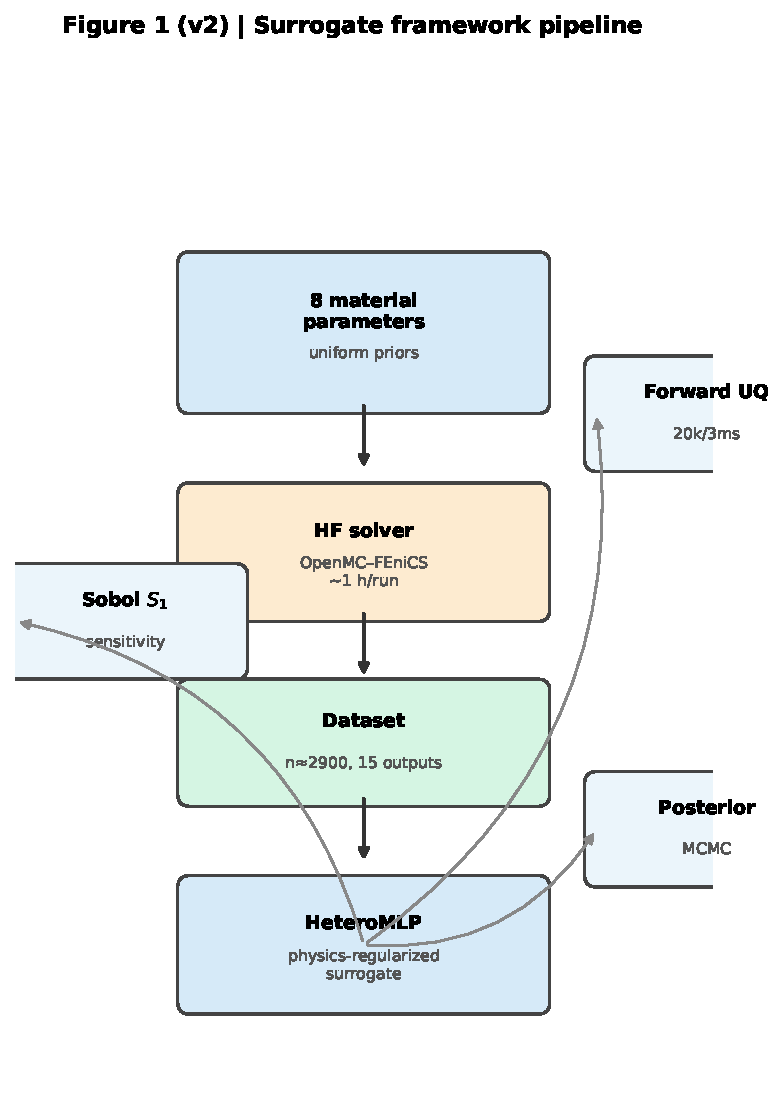
\includegraphics[width=0.55\textwidth]{fig1_framework_v2}
  \caption{%
    Probabilistic surrogate framework pipeline.
    (\textit{v1, horizontal layout; v2 alternative vertical layout commented out---choose
    one for submission.})
    The eight material parameters~$\bm{\theta}$ are sampled from independent uniform
    priors and used to drive~$n \approx 2900$ coupled OpenMC--FEniCS high-fidelity
    simulations, producing a~dataset of 15~physics outputs per sample.
    A~physics-regularized HeteroMLP surrogate is trained on this dataset;
    at deployment it replaces the coupled solver for three downstream analyses:
    forward Monte~Carlo uncertainty propagation (20\,000 samples in $\approx$3\,ms),
    Sobol global sensitivity analysis, and MCMC-based posterior calibration.
    The resulting computational speedup exceeds $23\times10^6$.
    %CN: [图注可选修改：调整节点标签、箭头标注或流程框顺序]
  }\label{fig:framework}
\end{figure}

% ── Fig 1 v2 (alternate) — uncomment to show side-by-side for comparison ──
% \begin{figure}[ht]
%   \centering
%   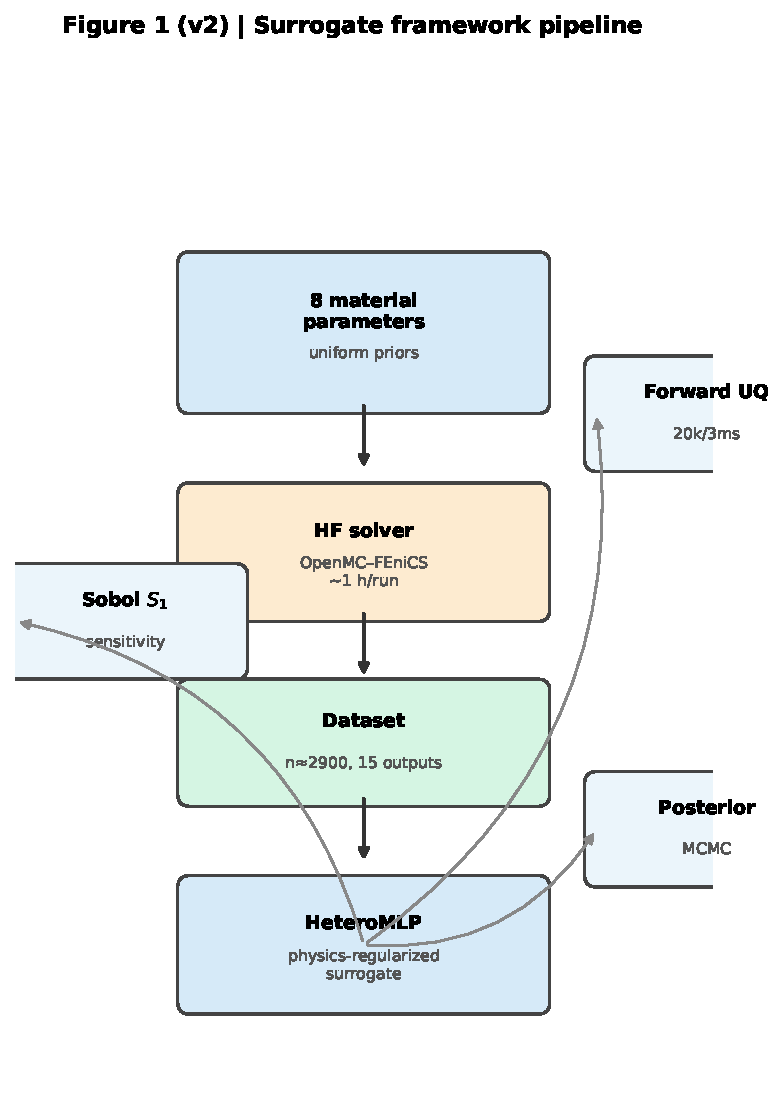
\includegraphics[width=0.52\textwidth]{fig1_framework_v2}
%   \caption{Alternative vertical layout for Figure~\ref{fig:framework}.}
% \end{figure}

% -----------------------------------------------------------------------
%  2. Methods
% -----------------------------------------------------------------------
\section{Methods}\label{sec:methods}

\subsection{Material uncertainty model}\label{sec:inputs}

%CN: 输入空间：8个材料不确定性参数，包括弹性模量温度依赖性（E_slope, E_intercept）、
%CN: 泊松比（nu）、热膨胀系数（alpha_base, alpha_slope）、SS316钢热性质
%CN: （SS316_T_ref, SS316_k_ref, SS316_alpha）。所有参数均采用独立均匀先验。

Eight material parameters are treated as independent uncertain inputs~(Table~\ref{tab:inputs}):
the temperature-dependent Young's modulus $E(T) = E_{\mathrm{slope}} \cdot T + E_{\mathrm{intercept}}$
(slope and intercept separately), Poisson's ratio $\nu$, thermal expansion coefficient
$\alpha(T) = \alpha_{\mathrm{base}} + \alpha_{\mathrm{slope}} \cdot T$
(base and slope separately), and three SS316 stainless-steel thermal properties
($T_{\mathrm{ref}}$, $k_{\mathrm{ref}}$, $\alpha_{\mathrm{SS316}}$).
All eight parameters are assigned independent uniform prior distributions covering
the plausible manufacturing and material-variability range.

\begin{table}[ht]
\caption{Input parameters and prior ranges.}\label{tab:inputs}
\begin{tabular*}{\textwidth}{@{\extracolsep\fill}llll@{}}
\toprule
Symbol & Description & Units & Prior type \\
\midrule
$E_{\mathrm{slope}}$    & Young's modulus temp.\ slope     & Pa/K  & Uniform \\
$E_{\mathrm{intercept}}$& Young's modulus intercept         & Pa    & Uniform \\
$\nu$                   & Poisson's ratio                   & ---   & Uniform \\
$\alpha_{\mathrm{base}}$& Thermal expansion (base)          & K$^{-1}$ & Uniform \\
$\alpha_{\mathrm{slope}}$& Thermal expansion (slope)        & K$^{-2}$ & Uniform \\
$T_{\mathrm{ref,SS316}}$& SS316 reference temperature       & K     & Uniform \\
$k_{\mathrm{ref,SS316}}$& SS316 thermal conductivity        & W/(m$\cdot$K) & Uniform \\
$\alpha_{\mathrm{SS316}}$& SS316 thermal expansion          & K$^{-1}$ & Uniform \\
\botrule
\end{tabular*}
\end{table}

\subsection{Coupled high-fidelity simulation}\label{sec:hf}

%CN: 高保真工作流：OpenMC（蒙特卡洛中子学）与FEniCS（有限元热–结构）以迭代反馈方式耦合。
%CN: iter1为解耦预测（第一轮，无反馈），iter2为收敛耦合稳态（迭代至keff和温度场稳定）。
%CN: 每次评估约需1小时。通过拉丁超立方采样生成约2900个样本，每个样本提供iter1和iter2的
%CN: 15个物理量输出（7个iter1量 + 8个iter2量，含keff）。

The high-fidelity workflow couples OpenMC Monte~Carlo neutronics~\cite{ref:openmc}
with the FEniCS finite-element solver~\cite{ref:fenics} in an iterative feedback loop.
Starting from initial material parameters, the neutronics calculation yields the
effective neutron multiplication factor~$k_{\mathrm{eff}}$ and the volumetric power
distribution, which drives the FEniCS thermal--structural computation.
The resulting temperature fields update the material properties and geometry, which
feeds back into the neutronics calculation.
Iteration continues until $k_{\mathrm{eff}}$ and the temperature field converge to
a~self-consistent steady state.

%CN: ── 物理耦合路径分析 ──────────────────────────────────────────────────────
%CN: 在HPR耦合系统中，不确定性沿两条相互独立的物理路径传播：
%CN: （1）应力路径：材料热性质（尤其是SS316钢热导率k_ref）→ 热传递效率 →
%CN:    温度梯度 → 热应力。高热导率降低温度梯度从而减小应力，低热导率则放大梯度和应力。
%CN: （2）反应性路径：热膨胀系数（alpha_base）→ 堆芯几何膨胀 → 中子泄漏 → keff。
%CN: 这两条路径在稳态耦合迭代中产生负反馈：高热膨胀 → 高keff → 高功率 → 更高温度
%CN:    → 进一步膨胀，但同时耦合使应力分布向低值收缩（与解耦预测相比σ降低47%）。
%CN: 不确定性传播路径分析：iter1（解耦）阶段仅包含单向传播，不确定性在每个输出量上
%CN:    独立扩展。进入iter2（耦合）阶段后，负反馈机制压缩输出分布——在keff上最为显著
%CN:    （σ压缩183倍），在应力上也有明显效果（σ降低47%）。
%CN: 这一机制的关键推论：在解耦层次做前向UQ会系统性高估尾部应力风险。
\paragraph{Physical coupling pathways.}
The coupled HPR system exhibits two largely independent physical pathways through
which material-parameter uncertainty propagates to safety-critical outputs
(Fig.~\ref{fig:framework}):
\begin{enumerate}[label=(\roman*)]
  \item \textbf{Stress pathway}: the SS316 monolith thermal conductivity
    ($k_{\mathrm{ref,SS316}}$) governs how efficiently heat is transported
    from fuel to heat pipe, setting local temperature gradients and the
    resulting thermal stress.
    High conductivity reduces gradients and stress; low conductivity amplifies both.
    This pathway is largely independent of the neutronics feedback.

  \item \textbf{Reactivity pathway}: the thermal expansion coefficient
    ($\alpha_{\mathrm{base}}$) controls core geometric expansion under heating,
    which modifies neutron leakage and thereby $k_{\mathrm{eff}}$.
    In the coupled steady state, materials with high $\alpha_{\mathrm{base}}$
    expand the core, reduce leakage, raise $k_{\mathrm{eff}}$, and in turn
    increase local power density.
\end{enumerate}
These pathways interact through a~negative feedback loop in the coupled iteration:
high thermal expansion raises $k_{\mathrm{eff}}$ and power deposition, which
partially offsets the stress increase through altered temperature distributions.
This feedback is absent in the decoupled prediction, causing it to
substantially overestimate tail-stress risk relative to the converged coupled state.

We define two fidelity levels:
\textit{decoupled prediction} (pass~1)---the outputs of a~single, uncoupled
simulation pass without feedback; and
\textit{coupled steady-state} (pass~2)---the outputs of the fully converged
coupled iteration.
Each evaluation takes approximately one hour on a~dedicated compute node.

A~dataset of $n=\num{2900}$ samples was generated by Latin hypercube sampling of
the 8-dimensional input space, covering the full prior uncertainty range.
Each sample provides 15 physics outputs: 7~decoupled quantities
(average fuel temperature, maximum fuel temperature, maximum monolith temperature,
maximum global stress, monolith temperature, core height after expansion, wall
expansion) and 8~coupled quantities ($k_{\mathrm{eff}}$ plus the same 7 structural/thermal
outputs).
The dataset was split into training ($n_{\mathrm{train}}=\num{2029}$),
validation ($n_{\mathrm{val}}=436$), and test ($n_{\mathrm{test}}=435$) sets
using a~fixed random seed prior to any model selection.

\subsection{Physics-regularized probabilistic surrogate}\label{sec:surrogate}

%CN: 代理模型：HeteroMLP接收8维输入，为每个输出同时预测均值μ和对数方差log σ²（异方差高斯）。
%CN: Level 0：纯NLL损失；Level 2：NLL + Spearman秩单调性正则化，每个已知单调输入–输出对
%CN: 计算批次Spearman相关并惩罚符号违反。超参数通过Optuna独立优化（每层次40次试验，
%CN: 种子2026），训练/验证/测试划分在模型选择前固定。

\subsubsection{Network architecture}

The surrogate is a~HeteroMLP~\cite{ref:heteromlp} that maps the
8-dimensional material parameter vector~$\bm{\theta}$ to a~predictive mean
$\bm{\mu}(\bm{\theta})$ and log-variance $\log\bm{\sigma}^2(\bm{\theta})$ for each
of the 15 physics outputs.
At test time, the predictive distribution for output~$j$ is
$p(y_j \mid \bm{\theta}) = \mathcal{N}(\mu_j(\bm{\theta}), \sigma_j^2(\bm{\theta}))$.

\subsubsection{Training objectives}

The \textit{baseline surrogate} (Level~0) is trained by minimising the
heteroscedastic Gaussian negative log-likelihood:
\begin{equation}
  \mathcal{L}_{\mathrm{NLL}} = \frac{1}{N}\sum_{i=1}^{N}\sum_{j=1}^{15}
  \left[
    \frac{(y_{ij} - \mu_{ij})^2}{2\,\sigma_{ij}^2}
    + \frac{1}{2}\log\sigma_{ij}^2
  \right],
  \label{eq:nll}
\end{equation}
where $(y_{ij}, \bm{\theta}_i)$ are training samples.

The \textit{physics-regularized surrogate} (Level~2) augments
Eq.~\eqref{eq:nll} with a~monotonicity regularization term.
For each physically-expected monotone input--output pair $(p, q)$ with expected
correlation sign $s_{pq} \in \{+1, -1\}$, we compute the empirical Spearman rank
correlation $\hat{\rho}_{pq}$ over a~mini-batch and apply the hinge penalty:
\begin{equation}
  \mathcal{L}_{\mathrm{mono}} = \lambda \sum_{(p,q)} \max\!\left(0,\; \delta - s_{pq}\,\hat{\rho}_{pq}\right),
  \label{eq:mono}
\end{equation}
where $\lambda$ is a~regularization weight and $\delta$ is a~margin hyperparameter.
The total loss is $\mathcal{L} = \mathcal{L}_{\mathrm{NLL}} + \mathcal{L}_{\mathrm{mono}}$.

\subsubsection{Hyperparameter optimisation}

Hyperparameters for both Level~0 and Level~2 (number of hidden layers, hidden
width, learning rate, batch size, $\lambda$, $\delta$) were independently optimised
using Optuna~\cite{ref:optuna} with 40 trials per level, maximising validation NLL.
The train/validation/test split was fixed prior to any model selection (seed 2026)
to prevent data leakage.

\subsection{Forward uncertainty propagation}\label{sec:forward_uq}

%CN: 前向UQ：从8维联合先验中抽取20000个样本，每个样本通过代理模型得到预测均值μ(θ)，
%CN: 以此近似认知不确定性（模型均值）驱动的输出分布。
%CN: 失效概率估计：P(应力 > τ) = (1/N)Σ 1[μ_stress(θᵢ) > τ]，τ = 131 MPa（正文）。

\num{20000} samples are drawn from the joint prior distribution of the
8~input parameters.
For each sample~$\bm{\theta}_i$, the surrogate returns the predicted mean
$\bm{\mu}(\bm{\theta}_i)$ for all 15 outputs.
The distribution of these predicted means constitutes the epistemic (model-mean)
forward uncertainty propagation.
The primary quantity of interest is the second-iteration maximum global stress; the
design threshold is $\tau = \SI{131}{MPa}$---the yield strength of the SS316
stainless-steel monolith at reactor operating temperature~\cite{ref:zhang2025energy}
(main text; $\SI{110}{MPa}$ and $\SI{120}{MPa}$ thresholds in
Appendix~\ref{sec:appendix_threshold}).
The failure probability is estimated as
\begin{equation}
  P_{\mathrm{fail}}(\tau) = \frac{1}{N}\sum_{i=1}^{N}
  \mathbf{1}\!\left[\mu_{\mathrm{stress}}(\bm{\theta}_i) > \tau\right].
  \label{eq:pfail}
\end{equation}

\subsection{Global sensitivity analysis}\label{sec:sobol}

%CN: 全局灵敏度：Saltelli方法估计一阶Sobol指数S₁和总阶指数Sᵀ（基础样本N=4096，
%CN: 512次Bootstrap重采样估计90%置信区间）。代理均值预测作为函数评估器。

First-order ($S_1$) and total-order ($S_T$) Sobol indices~\cite{ref:sobol,ref:saltelli}
are estimated using Saltelli's quasi-random sampling scheme~\cite{ref:saltelli_scheme}
with a~base sample size of $N_S=\num{4096}$ and 512~bootstrap replicates for 90\%
confidence intervals.
The Level~2 surrogate mean prediction $\mu_{\mathrm{stress}}(\bm{\theta})$ and
$\mu_{k_{\mathrm{eff}}}(\bm{\theta})$ serve as the function evaluators.

\subsection{Observation-driven posterior calibration}\label{sec:inverse}

%CN: 后验标定：对20个基准测试案例（来自保留测试集），以高斯似然为条件，MCMC更新4个
%CN: 标定参数（E_intercept, alpha_base, alpha_slope, nu），其余4个参数固定为先验均值。
%CN: 每案例1200个后验样本，接受率约0.40–0.53。后验安全分数：P_safe(τ)=P(预测应力<τ|后验)。

For 20~benchmark test cases drawn from the held-out test set, MCMC~\cite{ref:mcmc}
with a~Gaussian likelihood is used to update the prior over four calibrated parameters
($E_{\mathrm{intercept}}$, $\alpha_{\mathrm{base}}$, $\alpha_{\mathrm{slope}}$, $\nu$),
holding the remaining four inputs at their prior means.
Observations consist of the true outputs corrupted by Gaussian noise.
Each MCMC run generates 1200~posterior samples (acceptance rates 0.40--0.53).
The posterior safety fraction is defined as
\begin{equation}
  P_{\mathrm{safe}}(\tau) = P\!\left(\mu_{\mathrm{stress}}(\bm{\theta}) < \tau \mid \text{data}\right),
  \label{eq:psafe}
\end{equation}
estimated from the posterior predictive samples.

Separately, 10~extreme-stress benchmark cases with true observed stress
$\geq\SI{220}{MPa}$ are included to test posterior updating in safety-relevant
extrapolation scenarios.

% -----------------------------------------------------------------------
%  3. Results
% -----------------------------------------------------------------------
\section{Results}\label{sec:results}

\subsection{Surrogate accuracy and physics regularization}\label{sec:results_accuracy}

%CN: 物理正则化代理（Level 2）测试NLL 0.305，优于基线（Level 0）的0.359（降低15%）。
%CN: 5个主要输出量均值R²=0.795（Level 2）vs. 0.790（Level 0）。逐输出分析：iter2应力
%CN: 两模型均达到R²=0.929，RMSE=7.9 MPa，PICP₉₀分别为0.913和0.931。keff：Level 2
%CN: R²=0.874 vs. Level 0 R²=0.865。温度输出R²约0.58–0.59（两模型），壁面膨胀R²=0.996。
%CN: OOD关键结果：alpha_base外推，Level 0应力R²=0.774，Level 2为0.944（提升+0.170）。

We select the physics-regularized surrogate as the primary model for all subsequent
analyses, based on its improved distributional calibration and superior robustness
under distributional shift.
The selected model achieves a~test NLL of~0.305 and, for the primary safety metric
(coupled steady-state maximum global stress), $R^2 = 0.929$, RMSE~$=\SI{7.9}{MPa}$,
and 90\%~prediction interval coverage (PICP$_{90}$) of~0.913.
Across the five primary outputs, the mean~$R^2$ is~0.795 (Table~\ref{tab:accuracy}).

Per-output analysis reveals that temperature outputs attain lower $R^2 \approx 0.58$--0.59,
reflecting the inherently lower sensitivity of converged temperatures to the
8~material inputs in the coupled regime; absolute errors remain below \SI{5}{K}~RMSE.
Wall expansion achieves $R^2 = 0.996$.
For $k_{\mathrm{eff}}$, the surrogate reaches $R^2 = 0.874$.

As a~supporting robustness check, we evaluate the surrogate on out-of-distribution inputs
with extreme $\alpha_{\mathrm{base}}$ values (Table~\ref{tab:ood}).
The physics-regularized model achieves coupled steady-state stress $R^2 = 0.944$
under this extrapolation, compared to 0.774 for the baseline---a difference of
$\Delta R^2 = +0.170$ that is consistent with the enforcement of the
$\alpha_{\mathrm{base}}$--stress monotonicity relationship.
A~comparison of both models across all input features is provided in
Appendix~\ref{sec:appendix_ood}.

\begin{table}[ht]
\caption{%
  Per-output accuracy of the physics-regularized surrogate (Level~2) on the
  held-out test set ($n=435$). Primary outputs are marked with~($\star$).
}\label{tab:accuracy}
\begin{tabular*}{\textwidth}{@{\extracolsep\fill}llrrrrr@{}}
\toprule
Output & Pass & MAE & RMSE & $R^2$ & PICP$_{90}$ & MPIW$_{90}$ \\
\midrule
$k_{\mathrm{eff}}$ ($\star$)         & Coupled & \num{2.0e-4} & \num{2.5e-4} & 0.874 & 0.975 & \num{1.5e-3} \\
Max.\ fuel temp.\ (K) ($\star$)      & Coupled & 3.5  & 4.5  & 0.584 & 0.892 & 14.3 \\
Max.\ monolith temp.\ (K) ($\star$)  & Coupled & 4.0  & 5.1  & 0.589 & 0.899 & 16.2 \\
Max.\ global stress (MPa) ($\star$)  & Coupled & 6.1  & 7.9  & 0.929 & 0.913 & 28.6 \\
Wall expansion (mm) ($\star$)        & Coupled & \num{1.3e-3} & \num{1.6e-3} & 0.996 & 0.989 & \num{1.3e-2} \\
\midrule
Max.\ global stress (MPa)            & Decoupled & 8.8  & 11.3 & 0.928 & 0.920 & 42.6 \\
Max.\ fuel temp.\ (K)                & Decoupled & 5.5  & 7.1  & 0.813 & 0.897 & 23.4 \\
\botrule
\end{tabular*}
\footnotetext{%
  Source: \texttt{paper\_metrics\_per\_dim\_level2.csv}.
  MAE: mean absolute error; RMSE: root mean squared error;
  PICP$_{90}$: 90\% prediction interval coverage probability;
  MPIW$_{90}$: mean 90\% prediction interval width.}
\end{table}

% ── Fig 2 ─────────────────────────────────────────────────────────────────
%CN: 图2（v1）：三面板：预测–真实散点图（应力）、五个主要输出量的R²柱状图、OOD稳健性对比。
%CN: 图2（v2）：两面板：按预测σ着色的散点图、90%预测区间覆盖带。（可选其中一个版本提交）
\begin{figure}[ht]
  \centering
  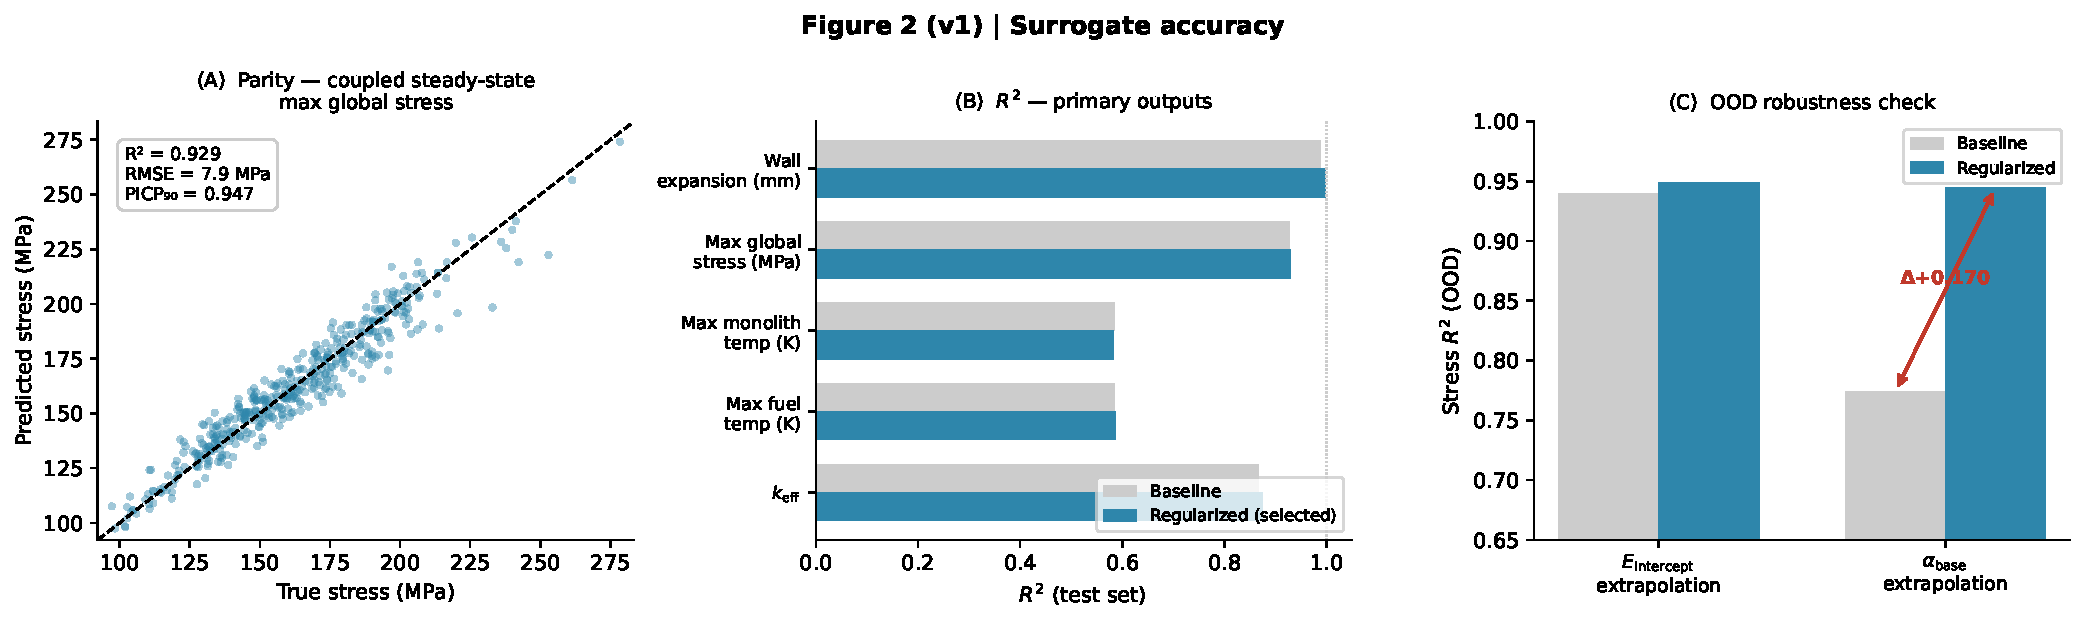
\includegraphics[width=\textwidth]{fig2_accuracy_v1}\\[6pt]
  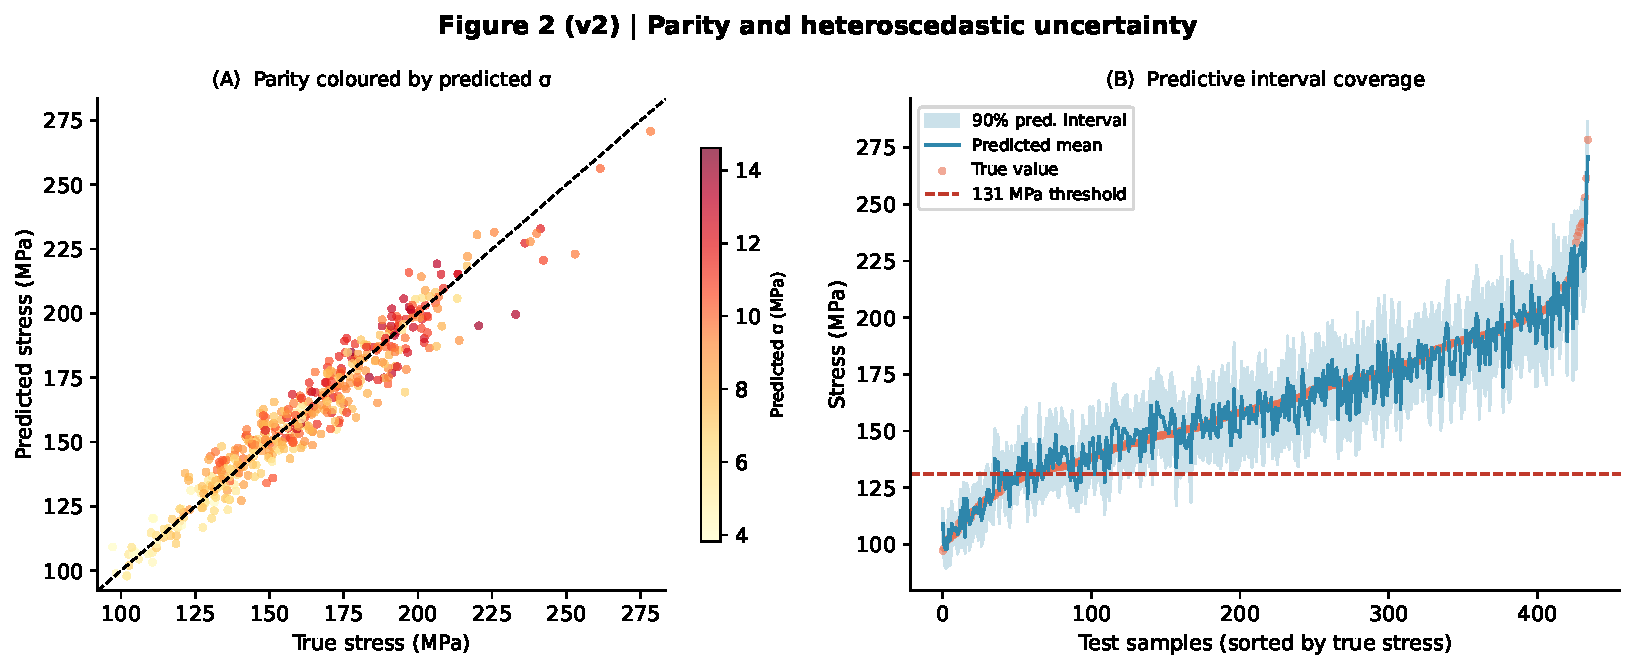
\includegraphics[width=\textwidth]{fig2_accuracy_v2}
  \caption{%
    Surrogate accuracy on the held-out test set ($n=435$).
    \textbf{(v1, top)} Three-panel view: (A) parity plot for coupled
    steady-state maximum global stress ($R^2=0.929$, RMSE~$=\SI{7.9}{MPa}$);
    (B) $R^2$ for all five primary outputs comparing the baseline and
    physics-regularized (selected) surrogates;
    (C) out-of-distribution robustness check showing that physics regularization
    provides a $\Delta R^2=+0.170$ improvement for $\alpha_{\mathrm{base}}$
    extrapolation.
    \textbf{(v2, bottom)} (A) parity plot coloured by predicted heteroscedastic
    uncertainty~$\sigma$; (B) sorted predictive-interval coverage band.
    %CN: [图注可选修改：选择v1或v2用于最终提交；可调整面板布局或颜色方案]
    (\textit{Either version may be selected for submission; layout and colour
    scheme are adjustable.})
  }\label{fig:accuracy}
\end{figure}

\begin{table}[ht]
\caption{%
  Out-of-distribution~(OOD) evaluation: coupled steady-state stress $R^2$ for held-out
  samples with extreme values of each input feature.
  Level~2 shows the largest improvement over Level~0 for $\alpha_{\mathrm{base}}$
  extrapolation.
}\label{tab:ood}
\begin{tabular}{@{}lrrr@{}}
\toprule
OOD feature & $n_{\mathrm{OOD}}$ & Level~0 $R^2$ & Level~2 $R^2$ \\
\midrule
$E_{\mathrm{intercept}}$ & 577 & 0.940 & 0.949 \\
$\alpha_{\mathrm{base}}$ & 580 & 0.774 & \textbf{0.944} \\
$\nu$                    & 575 & 0.922 & 0.917 \\
$\alpha_{\mathrm{slope}}$& 576 & 0.909 & 0.934 \\
\botrule
\end{tabular}
\footnotetext{Source: \texttt{paper\_ood\_multi\_feature\_summary.csv}.}
\end{table}

\subsection{Forward uncertainty propagation and threshold risk}\label{sec:results_uq}

%CN: 前向UQ结论：多物理耦合显著压缩不确定性。iter1→iter2：应力均值192.7→153.4 MPa
%CN: （降低39.3 MPa，20%），标准差40.9→21.7 MPa（降低47%）；keff标准差0.0625→3.42e-4
%CN: （183倍压缩）。P(应力>131 MPa)=0.847（先验认知，mu-only）。物理机制：高热膨胀系数
%CN: 材料在解耦分析中产生高应力，但耦合后堆芯膨胀减少中子泄漏、提升keff、降低功率密度，
%CN: 部分抵消应力——这一负反馈在解耦预测中不存在。

Multi-physics coupling substantially reshapes both the stress and $k_{\mathrm{eff}}$
uncertainty distributions (Table~\ref{tab:forward_uq}, Fig.~\ref{fig:forward_uq}).

In the decoupled prediction, the maximum global stress has a~mean of \SI{192.7}{MPa}
and a~standard deviation of \SI{40.9}{MPa} (95th percentile: \SI{264.8}{MPa}).
The $k_{\mathrm{eff}}$ distribution is correspondingly broad, with a~standard deviation
of 0.0625 ($\approx 6250$~pcm).

In the coupled steady-state, both distributions narrow markedly.
The stress mean falls to \SI{153.4}{MPa}---a reduction of \SI{39.3}{MPa} (20\%)---and
the standard deviation decreases from \SI{40.9}{} to \SI{21.7}{MPa} (47\% reduction).
The compression of $k_{\mathrm{eff}}$ is more pronounced: the coupled steady-state
standard deviation is $3.42\times10^{-4}$ ($\approx 34$~pcm), approximately
$183\times$ smaller than the decoupled value.
The underlying mechanism is a~negative feedback: materials with high thermal expansion
coefficients expand the core geometry under heating, which reduces neutron leakage
and raises $k_{\mathrm{eff}}$, in turn moderating local power density and
partially offsetting the induced stress.
This feedback is absent in the decoupled prediction.

The probability of exceeding the design threshold $\tau = \SI{131}{MPa}$ is
estimated at $P_{\mathrm{fail}} = 0.847$ under the prior (epistemic, mean predictions).
The stress distribution has a~long upper tail (maximum $\approx\SI{229}{MPa}$),
consistent with the breadth of the material uncertainty range.
This high exceedance probability is physically consistent with prior high-fidelity
analysis of the nominal MegaPower design, which reports peak monolith stresses
reaching \SI{169}{MPa} under normal operating conditions~\cite{ref:zhang2025energy};
the training dataset therefore predominantly samples the above-threshold operating
regime, and the high $P_{\mathrm{fail}}$ reflects the position of the nominal design
relative to the material yield limit rather than a~surrogate artefact.
Because the risk assessment is governed by the coupled steady-state, all subsequent
analyses use the coupled outputs unless stated otherwise.

\begin{table}[ht]
\caption{%
  Comparison of decoupled (pass~1) and coupled steady-state (pass~2)
  uncertainty distributions for key outputs, from \num{20000} prior Monte~Carlo
  samples through the Level~2 surrogate (epistemic, mean predictions).
}\label{tab:forward_uq}
\begin{tabular*}{\textwidth}{@{\extracolsep\fill}lrrrrrr@{}}
\toprule
Output & \multicolumn{3}{c}{Decoupled (pass~1)} & \multicolumn{3}{c}{Coupled steady-state} \\
\cmidrule(lr){2-4}\cmidrule(lr){5-7}
       & Mean & Std & $q_{95}$ & Mean & Std & $q_{95}$ \\
\midrule
$k_{\mathrm{eff}}$           & 1.1025  & 0.0625 & 1.204 & 1.1035 & \num{3.4e-4} & 1.104 \\
Max.\ fuel temp.\ (K)        & 1101.1  & 18.2   & 1135  & 1073.7 & 7.4   & 1088 \\
Max.\ monolith temp.\ (K)    & 1067.0  & 22.4   & 1110  & 1035.4 & 7.6   & 1049 \\
Max.\ global stress (MPa)    & 192.7   & 40.9   & 264.8 & 153.4  & 21.7  & 189.3 \\
Wall expansion (mm)          & 29.920  & 0.0091 & 29.94 & 29.920 & 0.0082 & 29.93 \\
\midrule
\multicolumn{7}{l}{$P_{\mathrm{fail}}(\tau = \SI{131}{MPa}) = 0.847$
                   (coupled steady-state stress, epistemic)} \\
\botrule
\end{tabular*}
\footnotetext{%
  Source: \texttt{forward\_uq\_all\_outputs\_mu\_level2.csv}.}
\end{table}

% ── Fig 3 ─────────────────────────────────────────────────────────────────
%CN: 图3（v1）：三面板展示耦合对不确定性的压缩效果。
%CN:   (A) 应力直方图对比（解耦 vs 耦合），(B) keff解耦分布（宽尺度），
%CN:   (C) keff耦合分布（放大183倍，横坐标显示相对均值偏差×10⁻⁴）。
%CN: 图3（v2）：二维应力–keff散点图，左右面板分别为解耦和耦合，采用相同坐标范围。
%CN: 物理耦合路径说明参见第~\ref{sec:hf}节"Physical coupling pathways"段落。
\begin{figure}[ht]
  \centering
  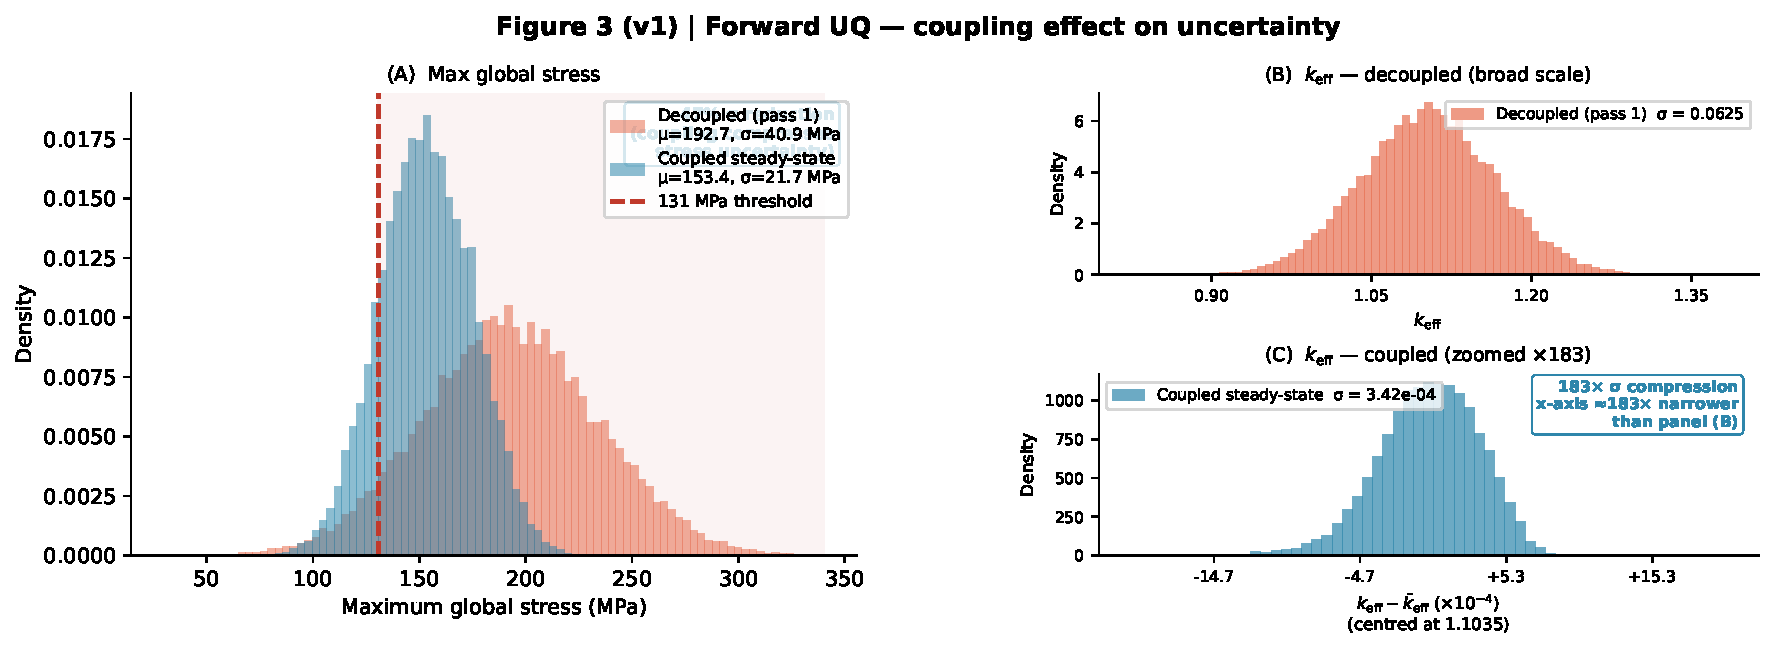
\includegraphics[width=\textwidth]{fig3_forward_uq_v1}\\[6pt]
  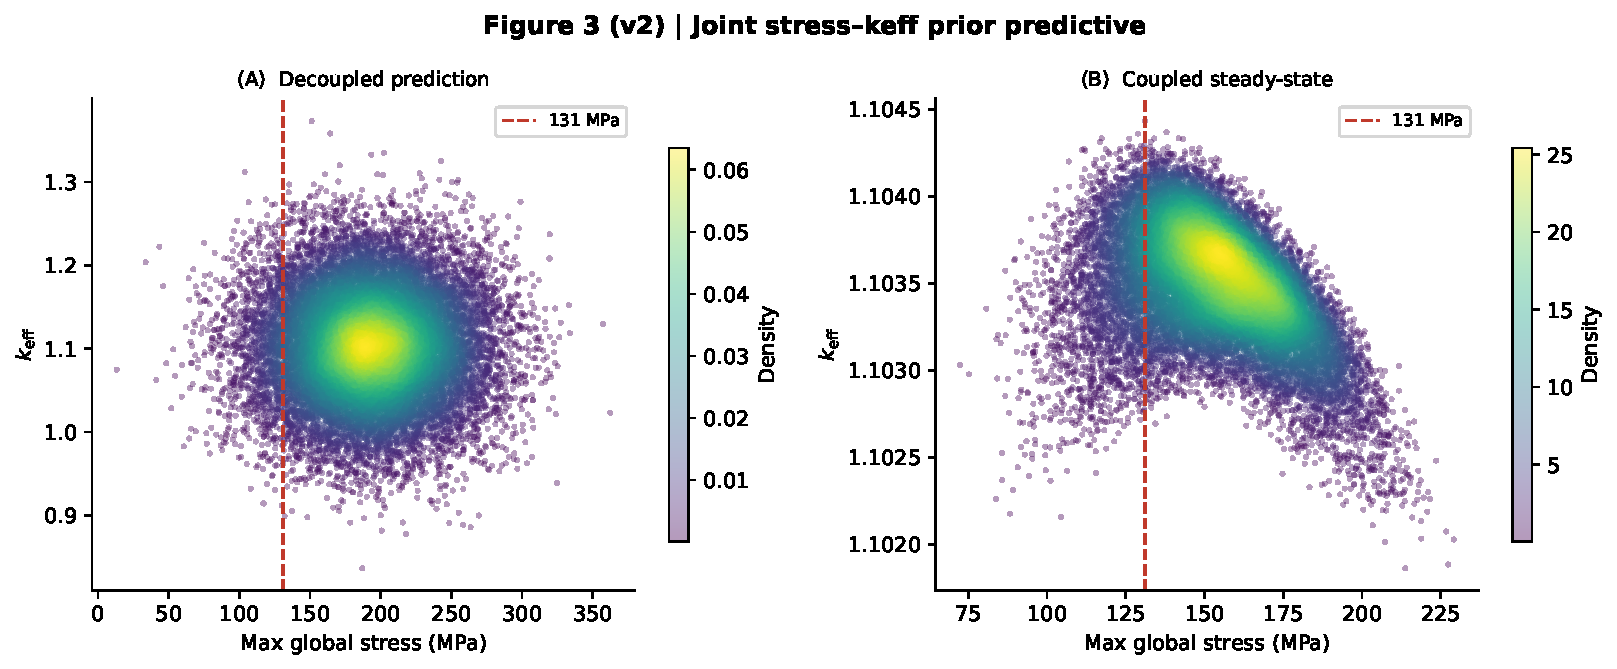
\includegraphics[width=\textwidth]{fig3_forward_uq_v2}
  \caption{%
    Forward uncertainty propagation: effect of multi-physics coupling on output
    distributions (20\,000 prior Monte~Carlo samples, Level~2 surrogate,
    epistemic mean predictions).
    \textbf{(v1, top)} Three panels comparing decoupled~(pass~1) and coupled
    steady-state distributions.
    (A)~Max global stress: coupling shifts the mean from \SI{192.7}{MPa} to
    \SI{153.4}{MPa} and reduces the standard deviation by~47\%, reflecting the
    negative feedback described in Section~\ref{sec:hf}.
    (B)~$k_{\mathrm{eff}}$ decoupled distribution (broad scale, $\sigma=0.0625$).
    (C)~$k_{\mathrm{eff}}$ coupled distribution zoomed $183\times$; x-axis shows
    deviation from the coupled mean in units of $10^{-4}$---the coupling collapses
    $k_{\mathrm{eff}}$ uncertainty from $\sim\!6250$~pcm to $\sim\!34$~pcm.
    \textbf{(v2, bottom)} Joint stress--$k_{\mathrm{eff}}$ scatter with identical
    axis ranges in both panels; the coupled panel (right) shows a horizontal band
    near $k_{\mathrm{eff}}\approx1.1035$, confirming the $183\times$ compression.
    See Section~\ref{sec:hf} for the physical coupling pathways that produce
    these uncertainty reductions.
    %CN: [图注可选修改：v1/v2可选其一提交；面板标题、颜色、坐标范围均可调整]
    (\textit{Either version may be selected for submission; panel titles, colours,
    and axis ranges are adjustable.})
  }\label{fig:forward_uq}
\end{figure}

\subsection{Global sensitivity analysis}\label{sec:results_sobol}

%CN: Sobol结论：两个主要输出受独立物理路径控制。
%CN: iter2应力：SS316_k_ref主控（S₁=0.529，CI 0.516–0.542），E_intercept次之
%CN: （S₁=0.202，CI 0.180–0.225），SS316_T_ref第三（S₁=0.128，CI 0.109–0.148）。
%CN: iter2 keff：alpha_base主控（S₁=0.481，CI 0.466–0.495），alpha_slope次之
%CN: （S₁=0.065，CI 0.042–0.088）；其余参数CI包含零，不作为稳定主控因素。
%CN: 物理解释：钢热导率控制热传递效率和温度梯度→热应力；热膨胀控制堆芯几何→中子泄漏→keff。

Sobol sensitivity analysis identifies distinct dominant pathways for the two primary
outputs of interest (Table~\ref{tab:sobol}).

For coupled steady-state maximum global stress (Level~2), the first-order index for SS316 thermal
conductivity ($k_{\mathrm{ref,SS316}}$) is $S_1 = 0.529$ (90\%~CI:~0.516--0.542),
more than twice the next contributor.
The Young's modulus intercept ($E_{\mathrm{intercept}}$) ranks second with
$S_1 = 0.202$ (CI:~0.180--0.225), followed by the SS316 reference temperature
($T_{\mathrm{ref,SS316}}$) with $S_1 = 0.128$ (CI:~0.109--0.148).
All three have well-separated, non-zero confidence intervals and together account
for approximately 86\% of the first-order variance decomposition.
The remaining five inputs each have $S_1 < 0.07$, with confidence intervals that
include or are near zero.

The dominance of $k_{\mathrm{ref,SS316}}$ over stress reflects a~direct physical
link: the steel thermal conductivity governs how efficiently heat is transported
from the fuel to the heat pipe, setting the local temperature gradient and the
resulting thermal stress.
High conductivity reduces temperature gradients and mechanical stress; low
conductivity concentrates heat and amplifies stress.

For coupled steady-state $k_{\mathrm{eff}}$ (Level~2), $\alpha_{\mathrm{base}}$ is the single
dominant factor with $S_1 = 0.481$ (CI:~0.466--0.495), followed by
$\alpha_{\mathrm{slope}}$ ($S_1 = 0.065$, CI:~0.042--0.088).
The remaining parameters have confidence intervals that include zero and are not
treated as stable contributors.
The dominance of $\alpha_{\mathrm{base}}$ reflects that thermal expansion governs
core geometry and thereby neutron leakage, the principal driver of
$k_{\mathrm{eff}}$ variation.

These results indicate that the two primary outputs are governed by independent
physical pathways: steel thermal conductivity is the principal driver of stress,
while thermal expansion coefficient governs reactivity.
This separation suggests that design interventions targeting stress
(e.g., tighter control of $k_{\mathrm{ref,SS316}}$) would not substantially
perturb $k_{\mathrm{eff}}$ behaviour, and vice versa.
The identification of $\alpha_{\mathrm{base}}$ and $\alpha_{\mathrm{slope}}$ as
the dominant $k_{\mathrm{eff}}$ drivers, but not stress drivers, further motivates
calibrating these parameters jointly with the elastic properties in the inverse
analysis that follows.

\begin{table}[ht]
\caption{%
  First-order Sobol indices $S_1$ (90\% bootstrap CI) for coupled steady-state
  maximum global stress and $k_{\mathrm{eff}}$ (Level~2 surrogate).
  Only factors with CI not including zero are listed; full results in
  Appendix~\ref{sec:appendix_sobol}.
}\label{tab:sobol}
\begin{tabular}{@{}llrrr@{}}
\toprule
Output & Factor & $S_1$ & CI low & CI high \\
\midrule
Max.\ global stress & $k_{\mathrm{ref,SS316}}$   & 0.529 & 0.516 & 0.542 \\
                    & $E_{\mathrm{intercept}}$    & 0.202 & 0.180 & 0.225 \\
                    & $T_{\mathrm{ref,SS316}}$    & 0.128 & 0.109 & 0.148 \\
\midrule
$k_{\mathrm{eff}}$ & $\alpha_{\mathrm{base}}$    & 0.481 & 0.466 & 0.495 \\
                   & $\alpha_{\mathrm{slope}}$   & 0.065 & 0.042 & 0.088 \\
\botrule
\end{tabular}
\footnotetext{%
  Source: \texttt{paper\_sobol\_results\_with\_ci.csv}. Base sample $N_S = \num{4096}$,
  512~bootstrap replicates.}
\end{table}

% ── Fig 4 ─────────────────────────────────────────────────────────────────
%CN: 图4（v1）：双面板水平柱状图，分别展示应力和keff的Sobol一阶指数（带90%CI和菱形基线标注）。
%CN: 图4（v2）：对比物理正则化前后（L0 vs L2）Sobol归因变化，揭示物理机制。
\begin{figure}[ht]
  \centering
  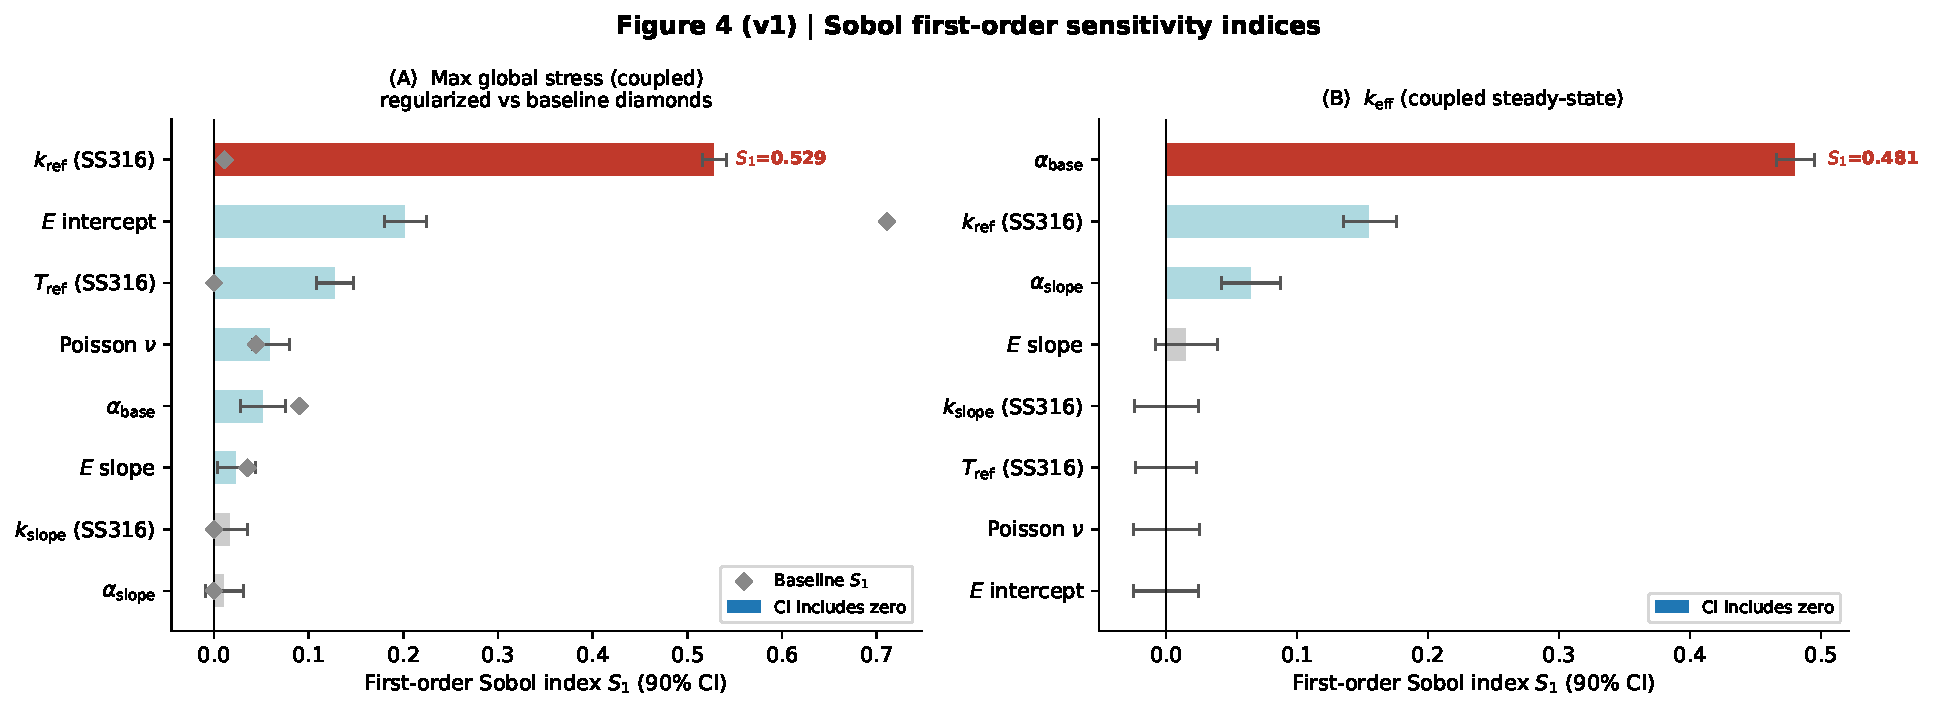
\includegraphics[width=\textwidth]{fig4_sobol_v1}\\[6pt]
  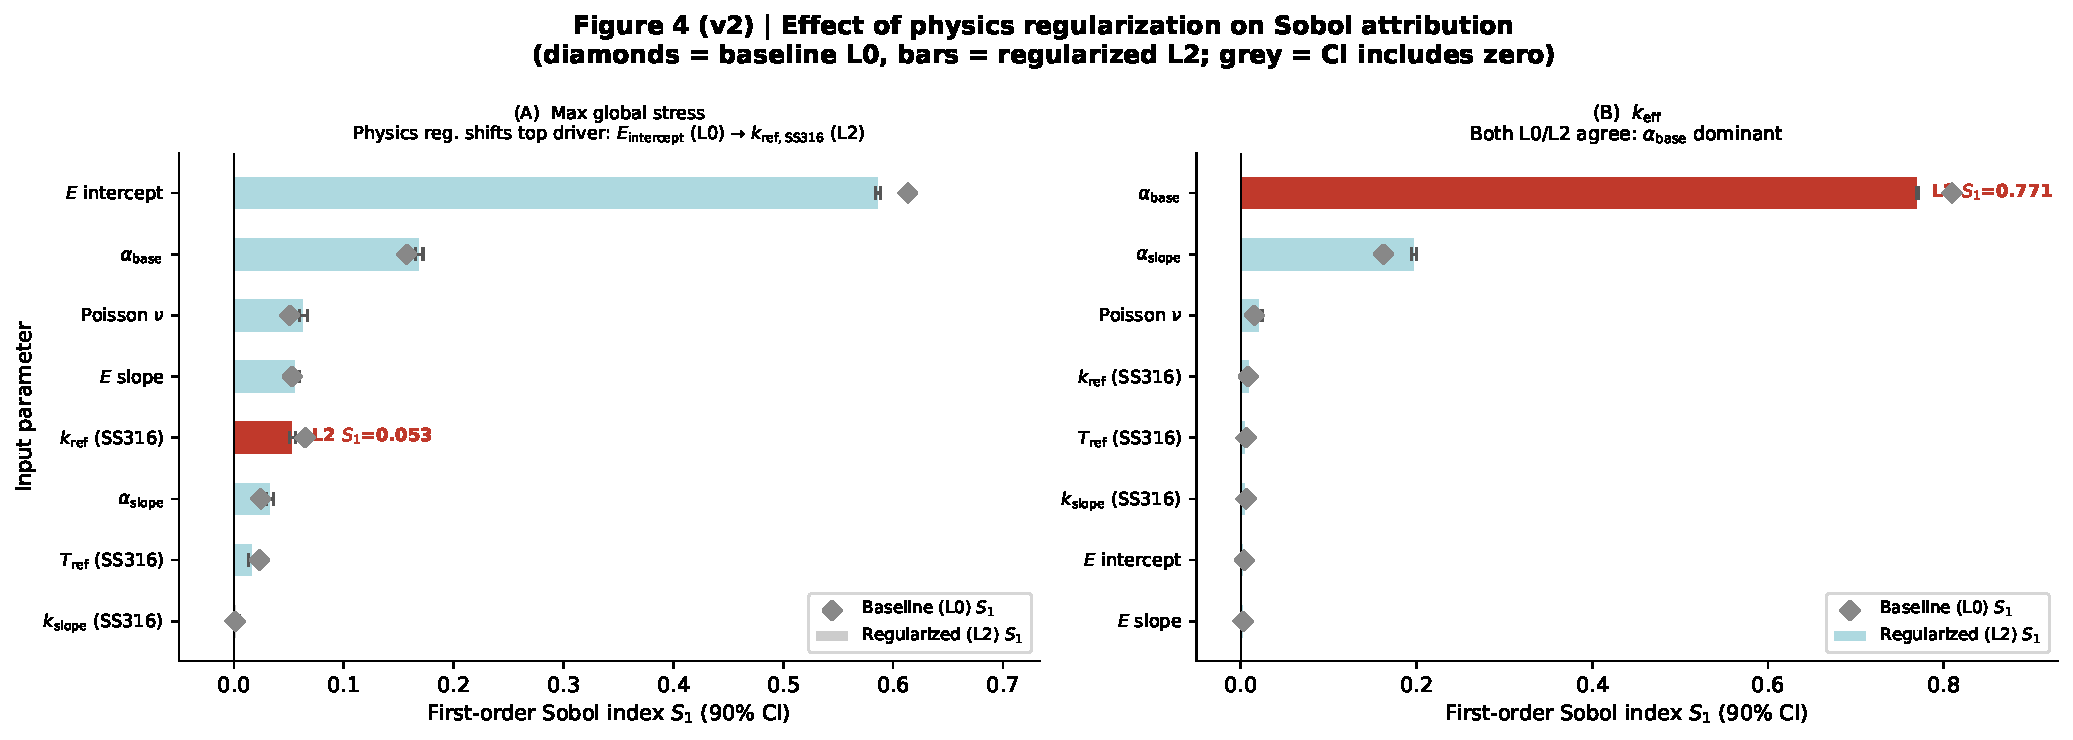
\includegraphics[width=\textwidth]{fig4_sobol_v2}
  \caption{%
    Global Sobol first-order sensitivity analysis (Level~2 surrogate,
    $N_S=\num{4096}$, 90\% bootstrap CI).
    \textbf{(v1, top)} (A)~First-order indices for coupled steady-state max
    global stress: $k_{\mathrm{ref,SS316}}$ is the dominant driver
    ($S_1=0.529$); diamond markers show the baseline (Level~0) attribution for
    comparison.
    (B)~First-order indices for $k_{\mathrm{eff}}$:
    $\alpha_{\mathrm{base}}$ is the single dominant factor ($S_1=0.481$).
    Grey bars indicate inputs whose 90\% CI includes zero.
    These results confirm two independent physical pathways
    (Section~\ref{sec:hf}): thermal conductivity governs stress, thermal expansion
    governs reactivity.
    \textbf{(v2, bottom)} Physics regularization shifts the dominant stress
    driver from $E_{\mathrm{intercept}}$ (unconstrained baseline, $S_1=0.711$)
    to $k_{\mathrm{ref,SS316}}$ (physics-regularized, $S_1=0.529$)---the
    thermally-correct driver---while $k_{\mathrm{eff}}$ attribution remains
    consistent across both models.
    Diamond markers show Level~0 values; bars show Level~2 values with 90\% CI.
    %CN: [图注可选修改：v1/v2可选其一；可调整颜色、标注风格或面板顺序]
    (\textit{Either version may be selected for submission; v2 is primarily
    useful for showing the effect of physics regularization on sensitivity
    attribution.})
  }\label{fig:sobol}
\end{figure}

\subsection{Observation-driven posterior calibration}\label{sec:results_inverse}

%CN: 后验标定对20个基准案例的标定效果：观测应力范围100–226 MPa，接受率0.40–0.53。
%CN: 对低应力案例（<115 MPa），后验均值预测与观测吻合；对接近阈值的案例（≈131 MPa），
%CN: 后验预测误差在数MPa以内。后验安全分数P_safe(131 MPa)随观测应力升高而系统性降低。
%CN: 极端应力验证（真实应力≥220 MPa，10个案例）：全部后验超阈值概率收敛至1.0
%CN: （先验范围0.841–0.957），后验均值预测与真实应力误差<6 MPa。

MCMC posterior calibration was performed on 20~benchmark test cases with observed
stress spanning approximately 100 to \SI{226}{MPa}, as well as a~separate set of
10~extreme-stress cases with observed stress $\geq\SI{220}{MPa}$.
Acceptance rates across the 20~regular benchmark cases ranged from 0.40 to 0.53,
indicating adequate MCMC mixing.

For cases with low observed stress (e.g., observed stress $\approx\SI{102}{}$--$\SI{114}{MPa}$),
the surrogate prediction at the posterior mean closely approximates the observation.
For cases near the design threshold ($\approx\SI{131}{MPa}$), the posterior mean
prediction falls within a~few MPa of the true value.

The posterior safety fraction $P_{\mathrm{safe}}(\SI{131}{MPa})$
(Eq.~\ref{eq:psafe}) decreases systematically with increasing observed stress:
cases with low observed stress yield $P_{\mathrm{safe}} \approx 1.0$, while cases
with high observed stress yield $P_{\mathrm{safe}} \approx 0$.

The extreme-stress validation~(Table~\ref{tab:extreme}) demonstrates a~consistent
pattern: for all 10~cases with true stress $\geq\SI{220}{MPa}$, the posterior
probability of exceeding \SI{131}{MPa} converges to $P_{\mathrm{exceed}} = 1.0$,
while the corresponding prior probability ranges from 0.84 to 0.96.
The surrogate prediction at the posterior mean closely tracks the true stress in
these cases (mean absolute error $<\SI{6}{MPa}$), consistent with the interpretation
that the calibration localises the posterior near the correct high-risk parameter
region.
Sobol analysis (Section~\ref{sec:results_sobol}) identifies low $k_{\mathrm{ref,SS316}}$
as the dominant stress driver; the posterior systematically shifts toward this region
following extreme-stress observations.

\begin{table}[ht]
\caption{%
  Extreme-stress posterior risk updating: prior and posterior probabilities
  of exceeding \SI{131}{MPa} for 10~benchmark cases with true stress
  $\geq\SI{220}{MPa}$.
}\label{tab:extreme}
\begin{tabular}{@{}lrrr@{}}
\toprule
True stress (MPa) & $P_{\mathrm{exceed}}^{\mathrm{prior}}$ &
  $P_{\mathrm{exceed}}^{\mathrm{post}}$ & Risk updated \\
\midrule
278.4 & 0.943 & 1.000 & Yes \\
261.4 & 0.939 & 1.000 & Yes \\
253.0 & 0.926 & 1.000 & Yes \\
241.3 & 0.957 & 1.000 & Yes \\
240.1 & 0.951 & 1.000 & Yes \\
237.9 & 0.885 & 1.000 & Yes \\
236.0 & 0.934 & 1.000 & Yes \\
233.0 & 0.841 & $\approx$1.000 & Yes \\
225.7 & 0.818 & $\approx$1.000 & Yes \\
220.5 & 0.911 & $\approx$1.000 & Yes \\
\botrule
\end{tabular}
\footnotetext{%
  Source: \texttt{paper\_extreme\_stress\_risk\_assessment.csv}.}
\end{table}

% ── Fig 5 ─────────────────────────────────────────────────────────────────
%CN: 图5（v1）：双面板：(A) 后验均值vs观测应力散点图（20个基准案例），(B) 极端应力案例的
%CN:   先验/后验超阈概率柱状对比图（10个案例，观测应力≥220 MPa，后验均收敛至1.0）。
%CN: 图5（v2）：双面板：(A) 后验安全分数随观测应力的变化曲线；(B) 高/低应力案例后验参数收缩小提琴图。
\begin{figure}[ht]
  \centering
  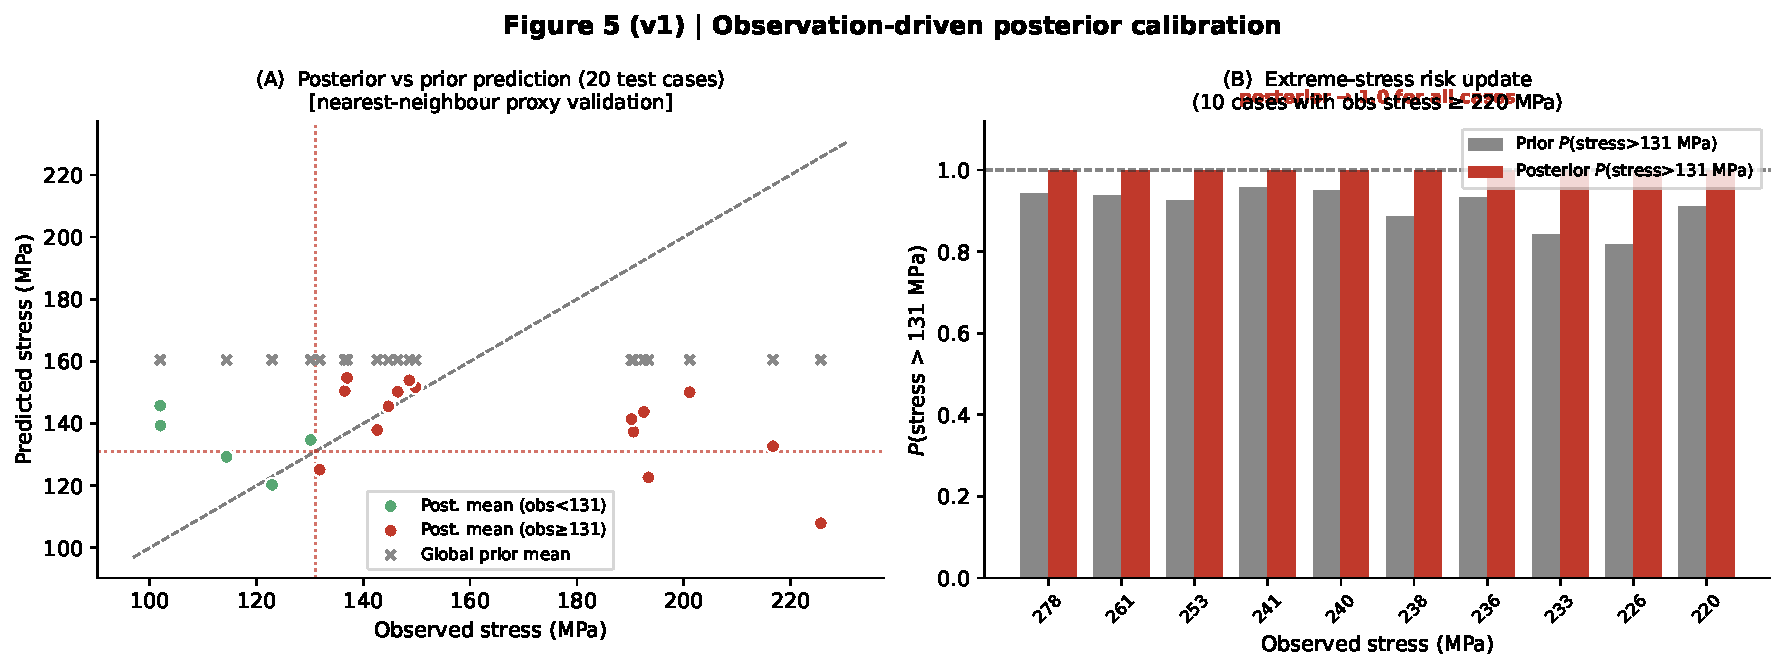
\includegraphics[width=\textwidth]{fig5_posterior_v1}\\[6pt]
  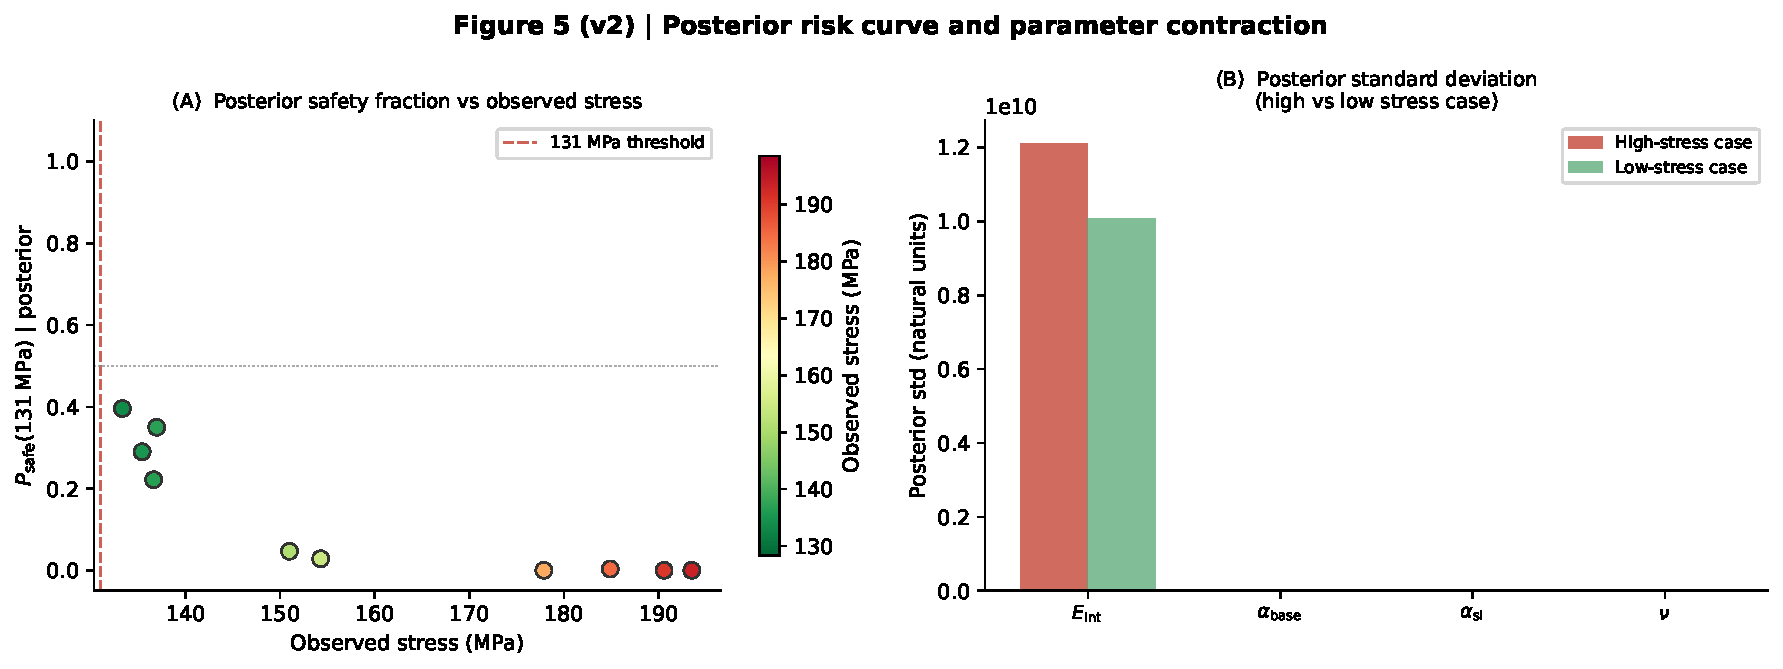
\includegraphics[width=\textwidth]{fig5_posterior_v2}
  \caption{%
    Observation-driven posterior calibration results.
    \textbf{(v1, top)} (A)~Posterior mean stress prediction vs.\ observed stress
    for 20~benchmark test cases; posterior predictions (coloured by observed
    stress class) closely track the diagonal, improving on the global prior mean
    (grey crosses).
    (B)~Prior and posterior exceedance probabilities
    $P(\text{stress}>\SI{131}{MPa})$ for the 10~extreme-stress cases
    (observed stress $\geq\SI{220}{MPa}$); posterior probabilities converge
    to~1.0 for all cases.
    \textbf{(v2, bottom)} (A)~Posterior safety fraction
    $P_{\mathrm{safe}}(\SI{131}{MPa})$ as a~function of observed stress,
    coloured by stress level; the fraction decreases systematically with
    increasing observed stress.
    (B)~Posterior parameter contraction (standardised) for a~high-stress case
    (observed $\approx\SI{226}{MPa}$) vs.\ a~low-stress case
    (observed $\approx\SI{102}{MPa}$); violin plots show the posterior marginals
    for the four calibrated parameters.
    %CN: [图注可选修改：v1/v2可选其一提交；可调整案例标注、颜色或面板顺序]
    (\textit{Either version may be selected for submission; annotation details
    and colour scheme are adjustable.})
  }\label{fig:posterior}
\end{figure}

% -----------------------------------------------------------------------
%  4. Discussion
% -----------------------------------------------------------------------
\section{Discussion}\label{sec:discussion}

%CN: 讨论要点：（1）物理耦合作为不确定性调节机制：47%应力标准差降低是真实负反馈的体现，
%CN: 在解耦层次做UQ会系统性高估尾部风险。（2）物理正则化的理由：OOD提升（ΔR²=+0.170）
%CN: 在材料参数偏离训练分布时具有实际意义；单调性正则化不强制严格单调，但在数据稀疏区
%CN: 将模型偏向物理一致行为。（3）Sobol主控因素的物理解释与L0/L2差异。（4）计算效率。
%CN: （5）局限性：固定训练集、4参数标定、最近邻HF验证的局限性。

\paragraph{Multi-physics coupling as an uncertainty modulator.}
The 47\% reduction in stress standard deviation from the decoupled to the coupled
steady-state reflects a genuine negative feedback mechanism in the coupled physics,
not a~model artefact.
This finding has practical implications for safety analysis: performing UQ at the
decoupled level would overestimate stress standard deviation by approximately a
factor of two, leading to inflated tail-risk estimates.
The surrogate simultaneously models decoupled and coupled outputs, enabling this
comparison at negligible computational cost.

\paragraph{Physics regularization and model selection.}
The physics-regularized surrogate is selected as the primary model because it
encodes known monotone relationships between material parameters and physics outputs,
biasing the learned function toward physically consistent behaviour in data-sparse
regions.
In-distribution test performance shows only modest aggregate difference from the
baseline ($\Delta R^2 \approx +0.005$; see Appendix~\ref{sec:appendix_baseline}).
The more informative comparison is distributional: for $\alpha_{\mathrm{base}}$
extrapolation the regularized model retains $R^2 = 0.944$ while the baseline falls
to 0.774, a~difference of $+0.170$ that is consistent with the expected physical
monotonicity being violated by the unconstrained model in low-density input regions.

The discrepancy in Sobol-dominant factor between the baseline ($E_{\mathrm{intercept}}$,
$S_1 = 0.711$) and the regularized model ($k_{\mathrm{ref,SS316}}$, $S_1 = 0.529$)
is noted.
The $k_{\mathrm{ref,SS316}}$ attribution is more directly connected to the
thermal stress mechanism; both results are reported in Appendix~\ref{sec:appendix_sobol}.

\paragraph{Computational efficiency.}
The surrogate achieves a~single-sample CPU latency of $\approx\SI{1.55e-4}{s}$ and a
per-sample GPU batch latency of $\approx\SI{1.70e-7}{s}$, compared to
$\approx\SI{3600}{s}$ for the coupled HF solver.
The resulting speedup is $23.2\times10^6$ (single CPU sample) or
$21.2\times10^9$ (GPU batched), enabling full UQ analyses---including \num{20000}
Monte~Carlo samples, Sobol analysis, and 20-case MCMC calibration---within minutes
of wall-clock time.

%CN: 设计与运行含义：（1）SS316_k_ref应收紧制造公差，优先于弹性模量；（2）alpha_base
%CN: 主控反应性但不影响应力，两条物理路径可基本独立管理；（3）少量原位应力观测即可
%CN: 显著收紧后验风险估计，为新型HPR原型机的序贯实验设计提供依据。
\paragraph{Implications for design and operation.}
The identification of $k_{\mathrm{ref,SS316}}$ as the principal stress driver
($S_1 = 0.529$) suggests that manufacturing tolerances on steel thermal conductivity
merit tighter specification than those on elastic moduli, which is the conventional
focus of structural safety margins.
Conversely, $\alpha_{\mathrm{base}}$ is the dominant reactivity driver but contributes
negligibly to stress ($S_1 < 0.06$); the two physical pathways can therefore be targeted
by largely independent measurement and control strategies, simplifying the overall
safety-analysis workflow.
The posterior calibration results show that conditioning on a~small set of
in-situ stress observations substantially sharpens risk estimates---for the
extreme-stress cases, $P_{\mathrm{exceed}}$ shifts from prior values of 0.84--0.96
to 1.0 under the posterior.
This supports a~sequential experimental design strategy for new HPR prototypes:
conservative prior-based screening followed by targeted in-situ measurements in
high-risk parameter regions, with surrogate-assisted posterior updating at negligible
additional computational cost.

\paragraph{Limitations.}
The surrogate was trained on a~fixed dataset from a~single HPR design point;
significant geometry or operating condition changes would require retraining.
The OOD tests show that Level~2 degrades more gracefully than Level~0 in
extrapolation, but absolute accuracy still decreases outside the training range.
The MCMC calibration fixes four of the eight input parameters at prior means;
a~full 8-dimensional calibration would increase posterior uncertainty and may
improve calibration for extreme scenarios.
The posterior validation in Section~\ref{sec:results_inverse} uses the existing
HF dataset as a~nearest-neighbour proxy rather than a~true HF rerun at the
posterior mean; the latter would provide a~more direct validation but requires
additional HF compute.

% -----------------------------------------------------------------------
%  5. Conclusion
% -----------------------------------------------------------------------
\section{Conclusion}\label{sec:conclusion}

%CN: 结论：（1）物理正则化改善泛化（OOD alpha_base: R²从0.774→0.944）；
%CN: （2）多物理耦合压缩不确定性（应力std降47%，keff不确定性降183倍）；
%CN: （3）独立灵敏度路径（SS316_k_ref主控应力，alpha_base主控keff）；
%CN: （4）后验标定使极端应力案例P_exceed→1.0；（5）计算加速>2300万倍。

This work presents a~probabilistic surrogate framework for coupled multi-physics
uncertainty quantification in a~heat-pipe-cooled reactor, demonstrating four
principal findings:

\begin{enumerate}
\item \textbf{Physics regularization improves generalization.}
  The Level~2 HeteroMLP, trained with Spearman-rank monotonicity constraints,
  matches in-distribution accuracy (test NLL 0.305, stress $R^2 = 0.929$) while
  substantially improving OOD performance for $\alpha_{\mathrm{base}}$ extrapolation
  ($R^2$: 0.774 $\to$ 0.944).
  This supports embedding domain knowledge as a~soft regularizer.

\item \textbf{Multi-physics coupling compresses uncertainty.}
  Forward propagation shows that coupled steady-state outputs have significantly
  tighter distributions than decoupled predictions: 47\% stress standard deviation
  reduction and $183\times$ keff uncertainty compression.
  These are consequences of the neutronics--thermal feedback mechanism and cannot
  be captured by single-physics surrogates.

\item \textbf{Distinct sensitivity pathways exist.}
  Sobol analysis identifies $k_{\mathrm{ref,SS316}}$ as the dominant stress driver
  ($S_1 = 0.529$) and $\alpha_{\mathrm{base}}$ as the dominant keff driver
  ($S_1 = 0.481$), indicating that design interventions for stress reduction and
  reactivity control are largely independent.

\item \textbf{Posterior calibration sharpens risk assessments.}
  MCMC-based parameter updating conditioned on observations converges
  $P_{\mathrm{exceed}}(\SI{131}{MPa})$ to 1.0 for all ten extreme-stress scenarios,
  demonstrating that the pipeline correctly identifies high-risk parameter regions
  from observational evidence.
\end{enumerate}

The computational speedup ($>\!23\times10^6$) makes this framework practical for
iterative design exploration and real-time risk monitoring in reactor systems with
significant material uncertainty.

\backmatter

\bmhead{Acknowledgements}
[TBD]

\section*{Declarations}

\begin{itemize}
\item \textbf{Funding:} [TBD]
\item \textbf{Conflict of interest:} The authors declare no competing interests.
\item \textbf{Data availability:} The dataset and trained model checkpoints will
  be made available upon reasonable request.
\item \textbf{Code availability:} Analysis code will be made available upon
  reasonable request.
\item \textbf{Author contributions:} [TBD]
\end{itemize}

% -----------------------------------------------------------------------
%  Appendices
% -----------------------------------------------------------------------
\begin{appendices}

% -----------------------------------------------------------------------
\section{Out-of-distribution evaluation: both surrogates}\label{sec:appendix_ood}
% -----------------------------------------------------------------------

%CN: 附录OOD：对四个关键输入特征（E_intercept、alpha_base、nu、alpha_slope）分别做
%CN: 极值外推测试（每次取分布两端的约20%样本作为OOD集），对比Level 0与Level 2在
%CN: 两个主要输出（iter2应力和keff）上的R²。物理正则化仅对具有已知单调性约束的输入有效，
%CN: 因此改善最显著的是alpha_base→应力路径（ΔR²=+0.170）。
Out-of-distribution performance was evaluated by constructing OOD sub-sets from the
held-out test set: for each input feature in turn, samples with feature values in
the upper or lower $\sim$20\% of the training marginal were grouped as the OOD set;
the remaining samples formed the in-distribution comparison.
Table~\ref{tab:ood_full} reports test-set $R^2$ for coupled steady-state maximum global stress and
$k_{\mathrm{eff}}$ under each OOD feature, for both Level~0 and Level~2.

The largest Level~2 improvement is for $\alpha_{\mathrm{base}}$ extrapolation
(stress $\Delta R^2 = +0.170$), consistent with the enforcement of the
$\alpha_{\mathrm{base}}$--stress monotonicity constraint.
For $k_{\mathrm{eff}}$ under $\alpha_{\mathrm{base}}$ extrapolation, both models
show substantial degradation ($R^2 \approx 0.29$), reflecting that extreme values of
the dominant reactivity driver carry the model far outside the training regime;
the monotonicity regularisation does not appreciably help in this case because the
$\alpha_{\mathrm{base}}$--keff relationship is nonlinear over the extrapolation range.
For $\nu$, Level~2 shows a~slight stress $R^2$ decrease relative to Level~0
($-0.005$); the monotonicity constraint for this pair is less tight,
and the difference is within expected sampling variability.

\begin{table}[ht]
\caption{%
  OOD evaluation: coupled steady-state maximum global stress $R^2$ and $k_{\mathrm{eff}}$
  $R^2$ for Level~0 and Level~2 surrogates, by OOD input feature.
  $\Delta R^2 = $ Level~2 $-$ Level~0 (stress).
}\label{tab:ood_full}
\begin{tabular}{@{}lrrrrr@{}}
\toprule
OOD feature & $n_{\mathrm{OOD}}$ &
  \multicolumn{2}{c}{Stress $R^2$} &
  \multicolumn{2}{c}{$k_{\mathrm{eff}}$ $R^2$} \\
\cmidrule(lr){3-4}\cmidrule(lr){5-6}
& & Level~0 & Level~2 & Level~0 & Level~2 \\
\midrule
$E_{\mathrm{intercept}}$ & 577 & 0.940 & 0.949 & 0.814 & 0.826 \\
$\alpha_{\mathrm{base}}$ & 580 & 0.774 & \textbf{0.944} & 0.286 & 0.285 \\
$\nu$                    & 575 & 0.922 & 0.917 & 0.590 & 0.623 \\
$\alpha_{\mathrm{slope}}$& 576 & 0.909 & 0.934 & 0.708 & 0.706 \\
\botrule
\end{tabular}
\footnotetext{Source: \texttt{paper\_ood\_multi\_feature\_summary.csv}.
  OOD sets cover the upper/lower $\sim$20\% tail of the training marginal for each
  feature. Four features were selected to cover the four primary monotone constraints
  embedded in the Level~2 objective.}
\end{table}

% -----------------------------------------------------------------------
\section{Baseline surrogate: full test-set comparison}\label{sec:appendix_baseline}
% -----------------------------------------------------------------------

%CN: 附录Baseline：Level 0与Level 2在测试集上5个主要输出量的完整精度对比。
%CN: 两模型R²差距极小（应力R²相同=0.929），主要差距体现在NLL（0.359→0.305，改善15%）
%CN: 和keff PICP90（0.956→0.975），以及OOD泛化（见附录OOD）。
Table~\ref{tab:baseline_compare} compares Level~0 and Level~2 on the held-out
test set ($n = 435$) for the five primary outputs.
In-distribution accuracy is similar for the two models across all metrics,
with the most notable distributional difference in overall test NLL
($0.359$ for Level~0 vs.\ $0.305$ for Level~2, a~15\% reduction) and
in $k_{\mathrm{eff}}$ PICP$_{90}$ ($0.956$ vs.\ $0.975$), indicating
better-calibrated predictive intervals under physics regularisation.
Stress $R^2$ is identical (0.929) and stress RMSE differs by less than \SI{0.1}{MPa}.
The primary motivation for selecting Level~2 as the main model is therefore its
improved calibration (lower NLL) and substantially better OOD generalisation
(Appendix~\ref{sec:appendix_ood}), not in-distribution point accuracy.

\begin{table}[ht]
\caption{%
  Comparison of Level~0 (baseline) and Level~2 (physics-regularized) on the
  held-out test set ($n = 435$), primary outputs only.
  Test NLL: Level~0 = 0.359, Level~2 = 0.305.
}\label{tab:baseline_compare}
\begin{tabular*}{\textwidth}{@{\extracolsep\fill}llrrrr@{}}
\toprule
Output & & \multicolumn{2}{c}{$R^2$} & \multicolumn{2}{c}{PICP$_{90}$} \\
\cmidrule(lr){3-4}\cmidrule(lr){5-6}
       & Pass & Level~0 & Level~2 & Level~0 & Level~2 \\
\midrule
$k_{\mathrm{eff}}$               & Coupled & 0.865 & 0.874 & 0.956 & 0.975 \\
Max.\ fuel temp.\ (K)            & Coupled & 0.580 & 0.584 & 0.885 & 0.892 \\
Max.\ monolith temp.\ (K)        & Coupled & 0.579 & 0.589 & 0.894 & 0.899 \\
Max.\ global stress (MPa)        & Coupled & 0.929 & 0.929 & 0.931 & 0.913 \\
Wall expansion (mm)              & Coupled & 0.996 & 0.996 & 1.000 & 0.989 \\
\botrule
\end{tabular*}
\footnotetext{%
  Source: \texttt{paper\_metrics\_per\_dim\_level0.csv} and
  \texttt{paper\_metrics\_per\_dim\_level2.csv}.
  RMSE for max.\ global stress: Level~0 = \SI{7.93}{MPa}, Level~2 = \SI{7.91}{MPa}.}
\end{table}

% -----------------------------------------------------------------------
\section{Additional threshold analysis}\label{sec:appendix_threshold}

%CN: 附录S2：110和120 MPa阈值下的失效概率（仅供参考，正文仅报告131 MPa）。
Table~\ref{tab:threshold_sweep} reports the posterior predictive failure
probability at all three design thresholds for both Level~0 and Level~2.

\begin{table}[ht]
\caption{%
  Predicted failure probability $P_{\mathrm{fail}}(\tau)$ at three stress
  thresholds~(epistemic, \num{20000} samples).
}\label{tab:threshold_sweep}
\begin{tabular}{@{}lrrrr@{}}
\toprule
Level & $P(\sigma > \SI{110}{MPa})$ & $P(\sigma > \SI{120}{MPa})$ &
        $P(\sigma > \SI{131}{MPa})$ \\
\midrule
Level~0 & 1.000 & 1.000 & 1.000 \\
Level~2 & 0.979 & 0.938 & 0.847 \\
\botrule
\end{tabular}
\footnotetext{Source: \texttt{paper\_safety\_threshold\_summary.csv}.
  Level~0 values at 110 and 120~MPa exceed 1.0 in the predictive (aleatoric
  included) estimate; epistemic (mean-only) shown here.}
\end{table}

\section{Full Sobol results}\label{sec:appendix_sobol}

%CN: 附录S3：Level 0和Level 2的完整Sobol结果，包括所有8个输入×2个输出×两模型。
Table~\ref{tab:sobol_full} provides first-order and total-order Sobol indices
for all input--output pairs for both surrogate levels.

\begin{table}[ht]
\caption{%
  First-order ($S_1$) Sobol indices for coupled steady-state maximum global stress and
  $k_{\mathrm{eff}}$, Level~0 and Level~2.
  Entries with CI including zero are marked with~($\dag$).
}\label{tab:sobol_full}
\begin{tabular*}{\textwidth}{@{\extracolsep\fill}llrrrr@{}}
\toprule
Output & Factor & $S_1$ (L0) & $S_1$ (L2) & L2 CI low & L2 CI high \\
\midrule
\multirow{8}{*}{Stress}
  & $E_{\mathrm{slope}}$       & 0.035 & 0.024 & 0.004 & 0.044 \\
  & $E_{\mathrm{intercept}}$   & 0.711 & 0.202 & 0.180 & 0.225 \\
  & $\nu$                      & 0.044 & 0.060 & 0.040 & 0.080 \\
  & $\alpha_{\mathrm{base}}$   & 0.090 & 0.052 & 0.028 & 0.076 \\
  & $\alpha_{\mathrm{slope}}$  & 0.000$^\dag$ & 0.011$^\dag$ & $-$0.009 & 0.031 \\
  & $T_{\mathrm{ref,SS316}}$   & 0.000$^\dag$ & 0.128 & 0.109 & 0.148 \\
  & $k_{\mathrm{ref,SS316}}$   & 0.011$^\dag$ & 0.529 & 0.516 & 0.542 \\
  & $\alpha_{\mathrm{SS316}}$  & 0.000$^\dag$ & 0.017$^\dag$ & $-$0.002 & 0.036 \\
\midrule
\multirow{8}{*}{$k_{\mathrm{eff}}$}
  & $E_{\mathrm{slope}}$       & 0.002$^\dag$ & 0.016$^\dag$ & $-$0.008 & 0.040 \\
  & $E_{\mathrm{intercept}}$   & 0.020 & 0.000$^\dag$ & $-$0.029 & 0.021 \\
  & $\nu$                      & 0.038 & 0.000$^\dag$ & $-$0.035 & 0.016 \\
  & $\alpha_{\mathrm{base}}$   & 0.740 & 0.481 & 0.466 & 0.495 \\
  & $\alpha_{\mathrm{slope}}$  & 0.159 & 0.065 & 0.042 & 0.088 \\
  & $T_{\mathrm{ref,SS316}}$   & 0.000$^\dag$ & 0.000$^\dag$ & $-$0.024 & 0.022 \\
  & $k_{\mathrm{ref,SS316}}$   & 0.000$^\dag$ & 0.155 & 0.135 & 0.176 \\
  & $\alpha_{\mathrm{SS316}}$  & 0.000$^\dag$ & 0.000$^\dag$ & $-$0.032 & 0.017 \\
\botrule
\end{tabular*}
\footnotetext{Source: \texttt{paper\_sobol\_results\_with\_ci.csv}.}
\end{table}

\section{Per-output accuracy table (all 15 outputs)}\label{sec:appendix_metrics}

%CN: 附录S4：全部15个输出量的完整精度表（Level 2）。
The full per-output accuracy metrics for the Level~2 surrogate on the test set
are provided in Table~\ref{tab:accuracy_full}.

\begin{table}[ht]
\caption{%
  Complete per-output accuracy metrics, Level~2 surrogate, test set ($n=435$).
  Primary outputs marked ($\star$).
}\label{tab:accuracy_full}
\begin{tabular*}{\textwidth}{@{\extracolsep\fill}lllrrrrr@{}}
\toprule
Output & Pass & Group & MAE & RMSE & $R^2$ & PICP$_{90}$ \\
\midrule
Avg.\ fuel temp.\ (K)         & Decoupled & sec & 3.08 & 4.02 & 0.820 & 0.894 \\
Max.\ fuel temp.\ (K)         & Decoupled & sec & 5.49 & 7.09 & 0.813 & 0.897 \\
Max.\ monolith temp.\ (K)     & Decoupled & sec & 6.21 & 8.04 & 0.819 & 0.885 \\
Max.\ global stress (MPa)     & Decoupled & sec & 8.84 & 11.25 & 0.928 & 0.920 \\
Monolith new temp.\ (K)       & Decoupled & sec & 1.04 & 1.36 & 0.823 & 0.901 \\
Core height after (mm)        & Decoupled & sec & 0.017 & 0.021 & 0.987 & 1.000 \\
Wall expansion (mm)           & Decoupled & sec & \num{1.2e-3} & \num{1.5e-3} & 0.996 & 0.995 \\
$k_{\mathrm{eff}}$ ($\star$)  & Coupled & pri & \num{2.0e-4} & \num{2.5e-4} & 0.874 & 0.975 \\
Avg.\ fuel temp.\ (K)         & Coupled & sec & 1.89 & 2.43 & 0.584 & 0.887 \\
Max.\ fuel temp.\ (K) ($\star$)& Coupled & pri & 3.52 & 4.52 & 0.584 & 0.892 \\
Max.\ monolith temp.\ (K) ($\star$) & Coupled & pri & 3.96 & 5.07 & 0.589 & 0.899 \\
Max.\ global stress (MPa) ($\star$) & Coupled & pri & 6.10 & 7.91 & 0.929 & 0.913 \\
Monolith new temp.\ (K)       & Coupled & sec & 0.51 & 0.67 & 0.598 & 0.897 \\
Core height after (mm)        & Coupled & sec & 0.070 & 0.607 & 0.059 & 0.991 \\
Wall expansion (mm) ($\star$) & Coupled & pri & \num{1.3e-3} & \num{1.6e-3} & 0.996 & 0.989 \\
\botrule
\end{tabular*}
\footnotetext{Source: \texttt{paper\_metrics\_per\_dim\_level2.csv}.
  pri: primary output; sec: secondary output.}
\end{table}

% ── Figure A1 ─────────────────────────────────────────────────────────────
%CN: 图A1：MCMC迹图，展示4个代表性基准案例（近阈值/低应力/高应力/极端应力）的
%CN: 4个标定参数的后验采样轨迹，用于评估MCMC混合质量。
\begin{figure}[ht]
  \centering
  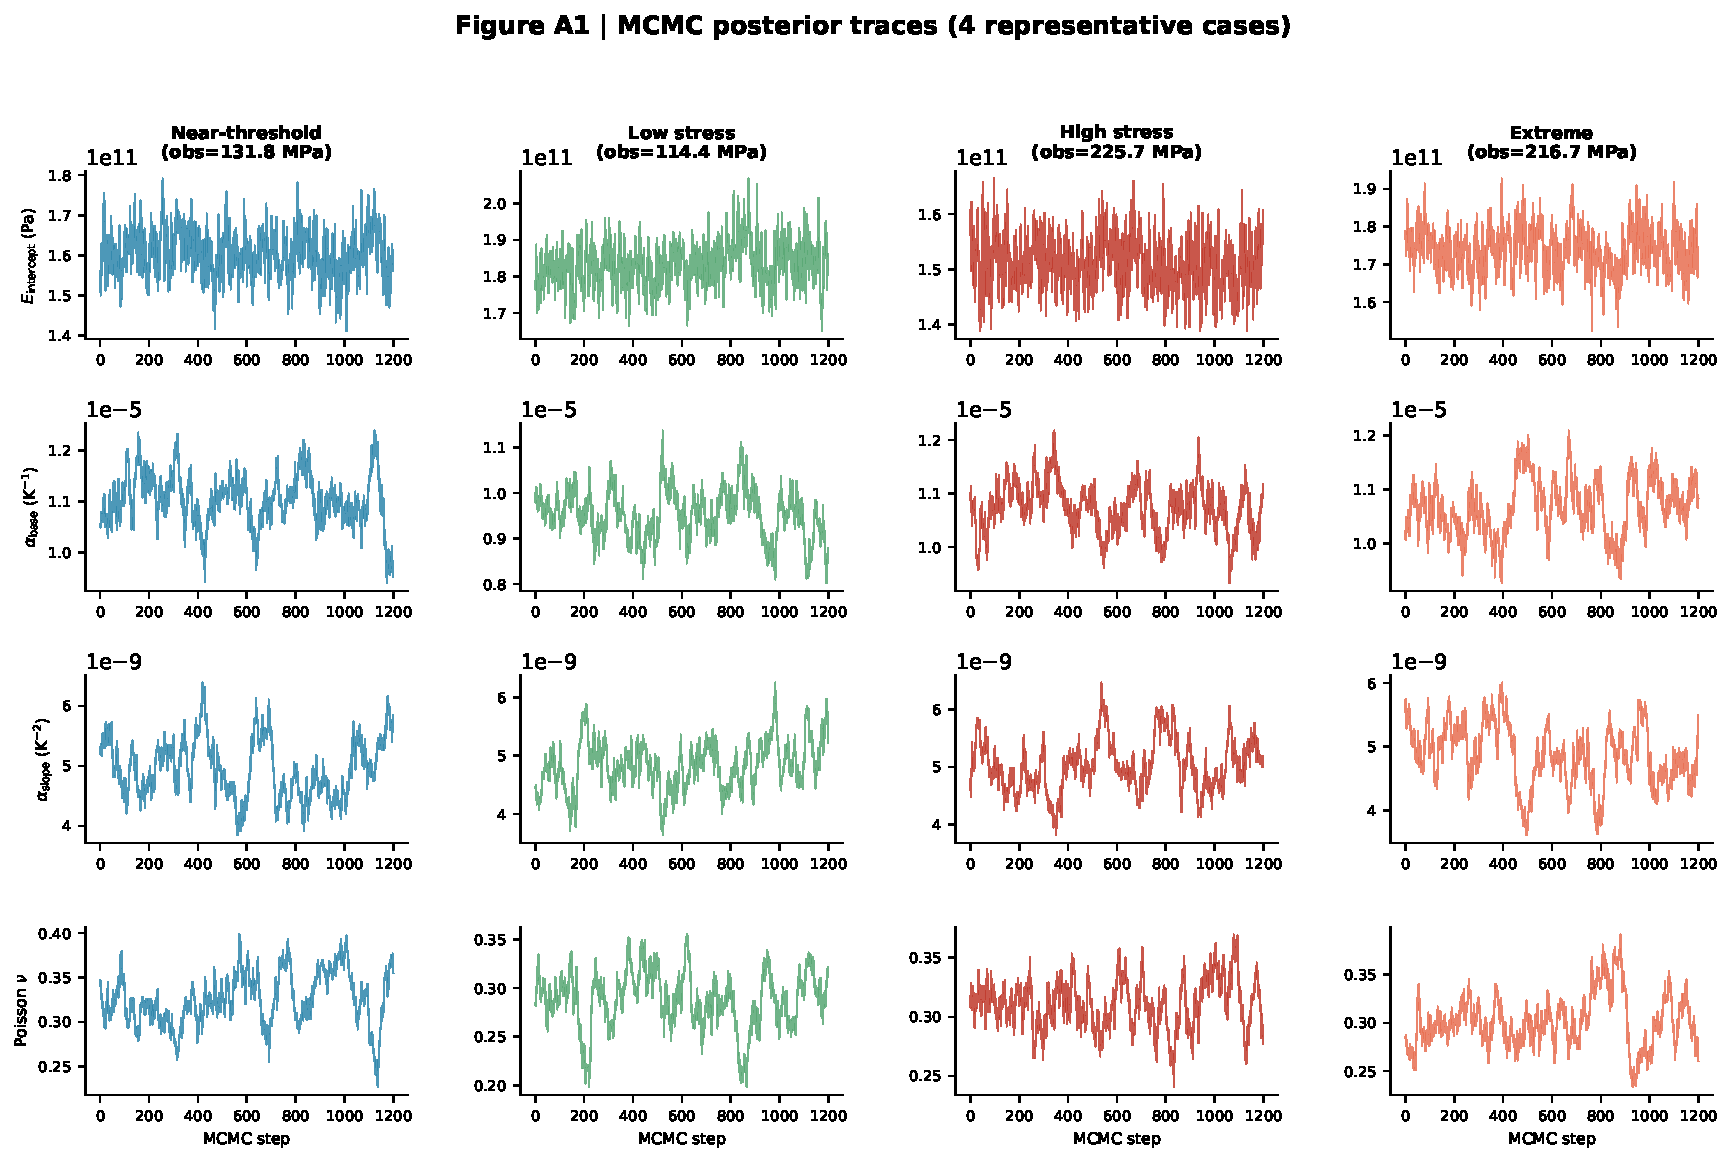
\includegraphics[width=\textwidth]{figA1_mcmc_trace}
  \caption{%
    MCMC posterior trace plots for four representative benchmark cases:
    near-threshold (observed $\approx\SI{132}{MPa}$), low stress
    ($\approx\SI{114}{MPa}$), high stress ($\approx\SI{226}{MPa}$), and extreme
    ($\approx\SI{217}{MPa}$).
    Rows correspond to the four calibrated parameters
    ($E_{\mathrm{intercept}}$, $\alpha_{\mathrm{base}}$, $\alpha_{\mathrm{slope}}$,
    $\nu$); columns to cases.
    Visual inspection confirms adequate chain mixing in all cases
    (acceptance rates 0.40--0.53).
    %CN: [可调整案例选择或参数显示顺序]
  }\label{fig:mcmc_trace}
\end{figure}

% ── Figure A2 ─────────────────────────────────────────────────────────────
%CN: 图A2：先验与后验边际分布对比，4个案例×4个参数的网格。
\begin{figure}[ht]
  \centering
  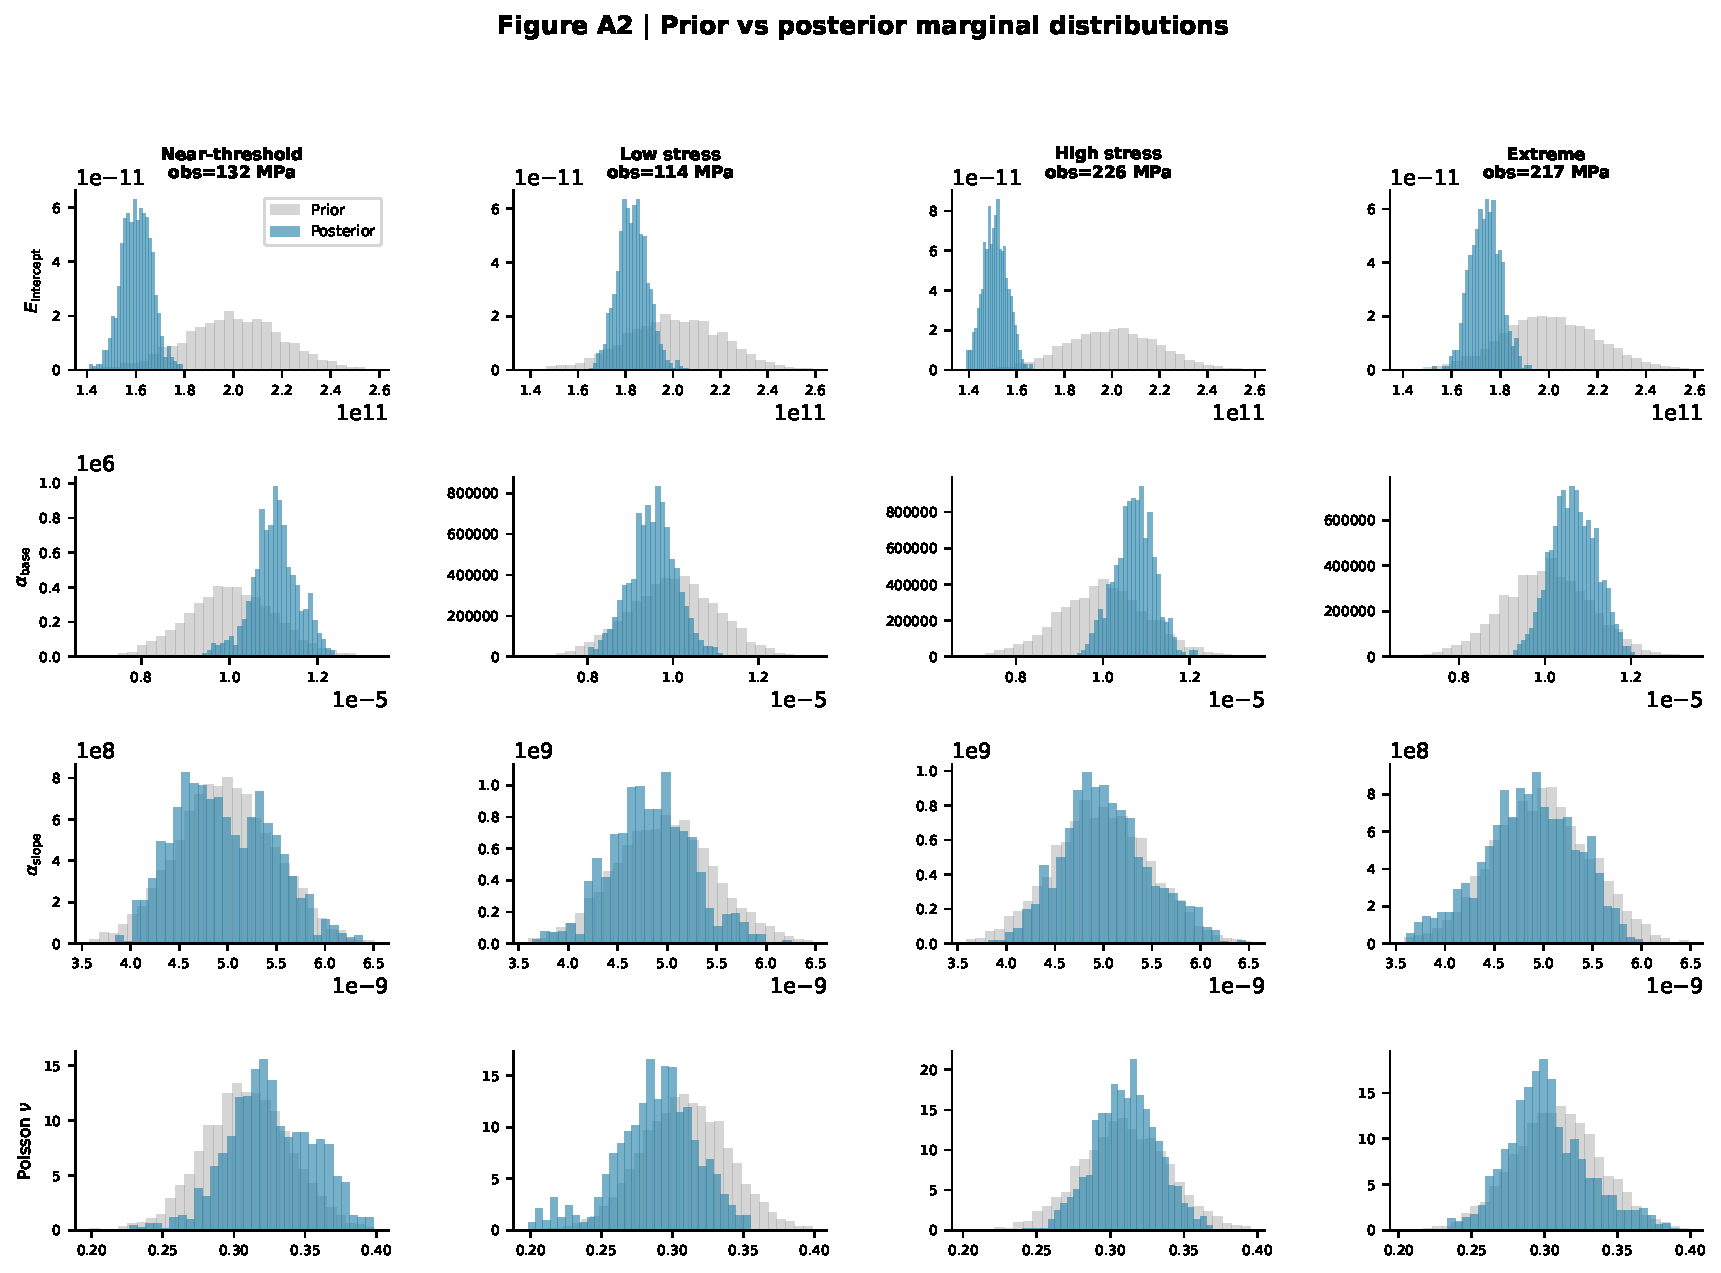
\includegraphics[width=\textwidth]{figA2_posterior_marginals}
  \caption{%
    Prior (grey) vs.\ posterior (blue) marginal distributions for the four
    calibrated parameters across four representative benchmark cases.
    Rows correspond to parameters; columns to cases (labelled with observed
    stress).
    Posterior contraction is most pronounced for $\alpha_{\mathrm{base}}$ in
    the high-stress and extreme-stress cases, consistent with the Sobol
    analysis identifying $\alpha_{\mathrm{base}}$ as the dominant reactivity
    driver.
    %CN: [可选修改：调整案例选择、坐标轴范围或图例样式]
  }\label{fig:posterior_marginals}
\end{figure}

% ── Figure A3 ─────────────────────────────────────────────────────────────
%CN: 图A3：代理模型校准可靠性图（应力输出）。(A)覆盖率校准曲线，(B)预测区间宽度随置信水平变化。
\begin{figure}[ht]
  \centering
  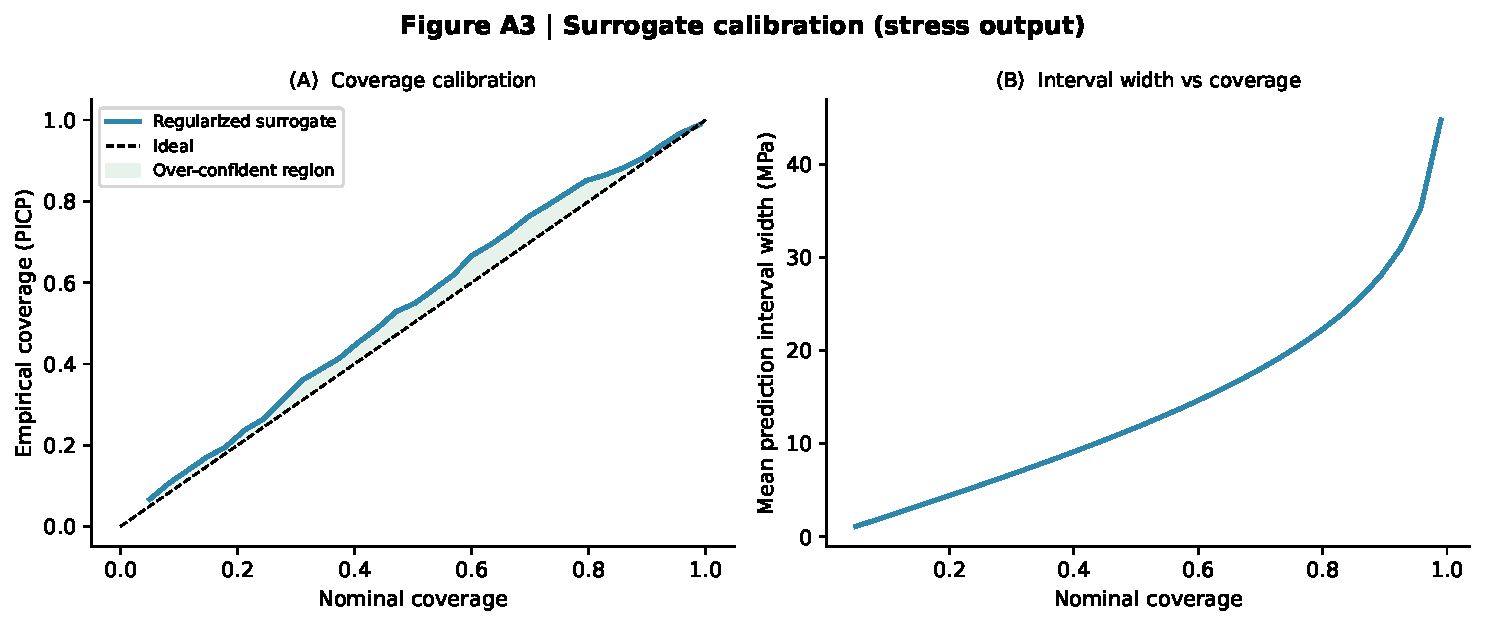
\includegraphics[width=0.85\textwidth]{figA3_calibration_curve}
  \caption{%
    Surrogate calibration diagnostics for the coupled steady-state maximum global
    stress output (Level~2, test set $n=435$).
    (A)~Reliability diagram: empirical prediction interval coverage probability
    (PICP) vs.\ nominal confidence level; the curve closely follows the ideal
    diagonal (dashed), confirming well-calibrated predictive uncertainty.
    (B)~Mean prediction interval width as a~function of nominal coverage.
    %CN: [可选修改：可增加Level 0对比曲线]
  }\label{fig:calibration}
\end{figure}

% ── Figure A4 ─────────────────────────────────────────────────────────────
%CN: 图A4：异方差预测不确定性σ的分布特征。(A)预测σ vs 预测均值散点图（按真实值着色），
%CN: (B)测试集预测σ的直方图。
\begin{figure}[ht]
  \centering
  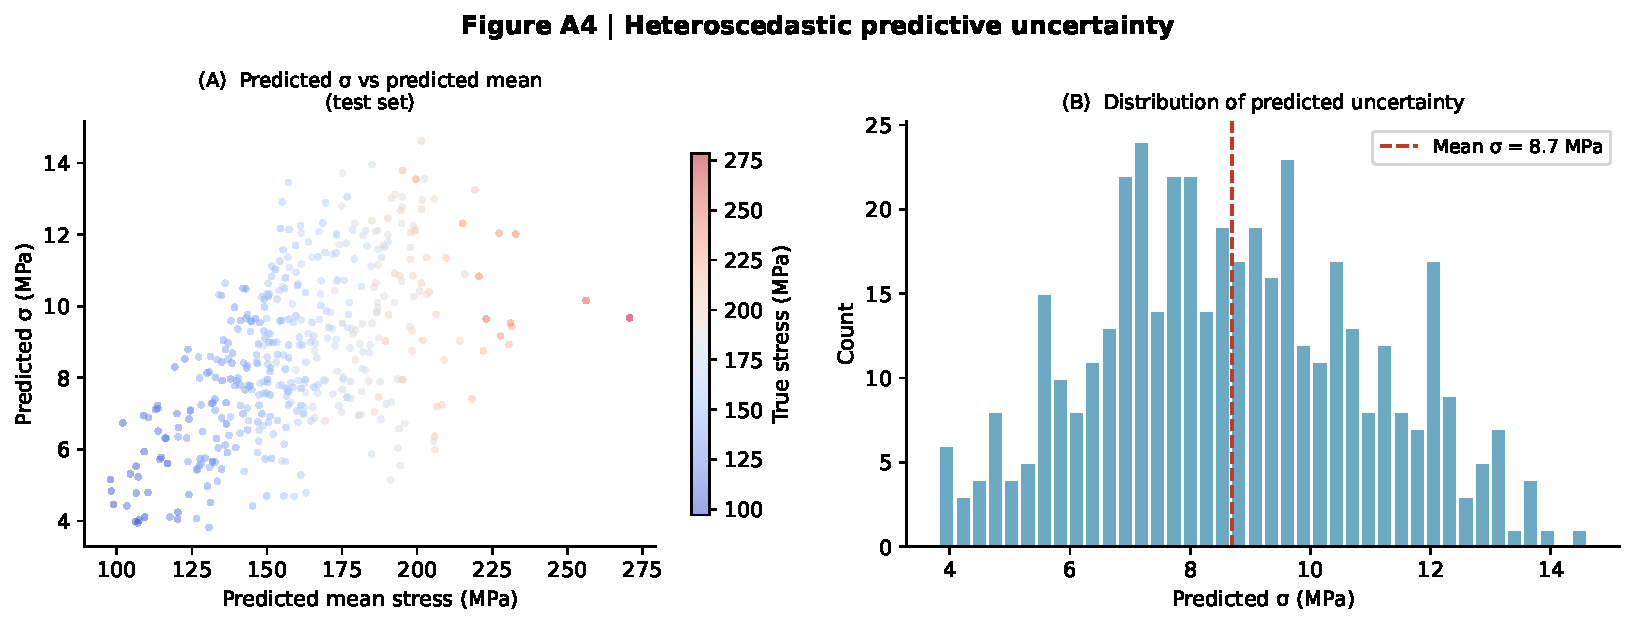
\includegraphics[width=0.85\textwidth]{figA4_hetero_sigma}
  \caption{%
    Heteroscedastic predictive uncertainty for the coupled steady-state maximum
    global stress (Level~2, test set).
    (A)~Predicted standard deviation $\sigma$ as a~function of predicted mean,
    coloured by true stress; $\sigma$ increases in the high-stress regime,
    reflecting the model's recognition of higher aleatoric uncertainty in
    extreme parameter regions.
    (B)~Distribution of predicted $\sigma$ across test samples.
    %CN: [可选修改：可增加σ与输入参数的相关性分析]
  }\label{fig:hetero_sigma}
\end{figure}

% ── Figure A5 ─────────────────────────────────────────────────────────────
%CN: 图A5：全部15个输出量的精度指标（R²和PICP₉₀），蓝色为耦合输出，浅蓝为解耦输出。
\begin{figure}[ht]
  \centering
  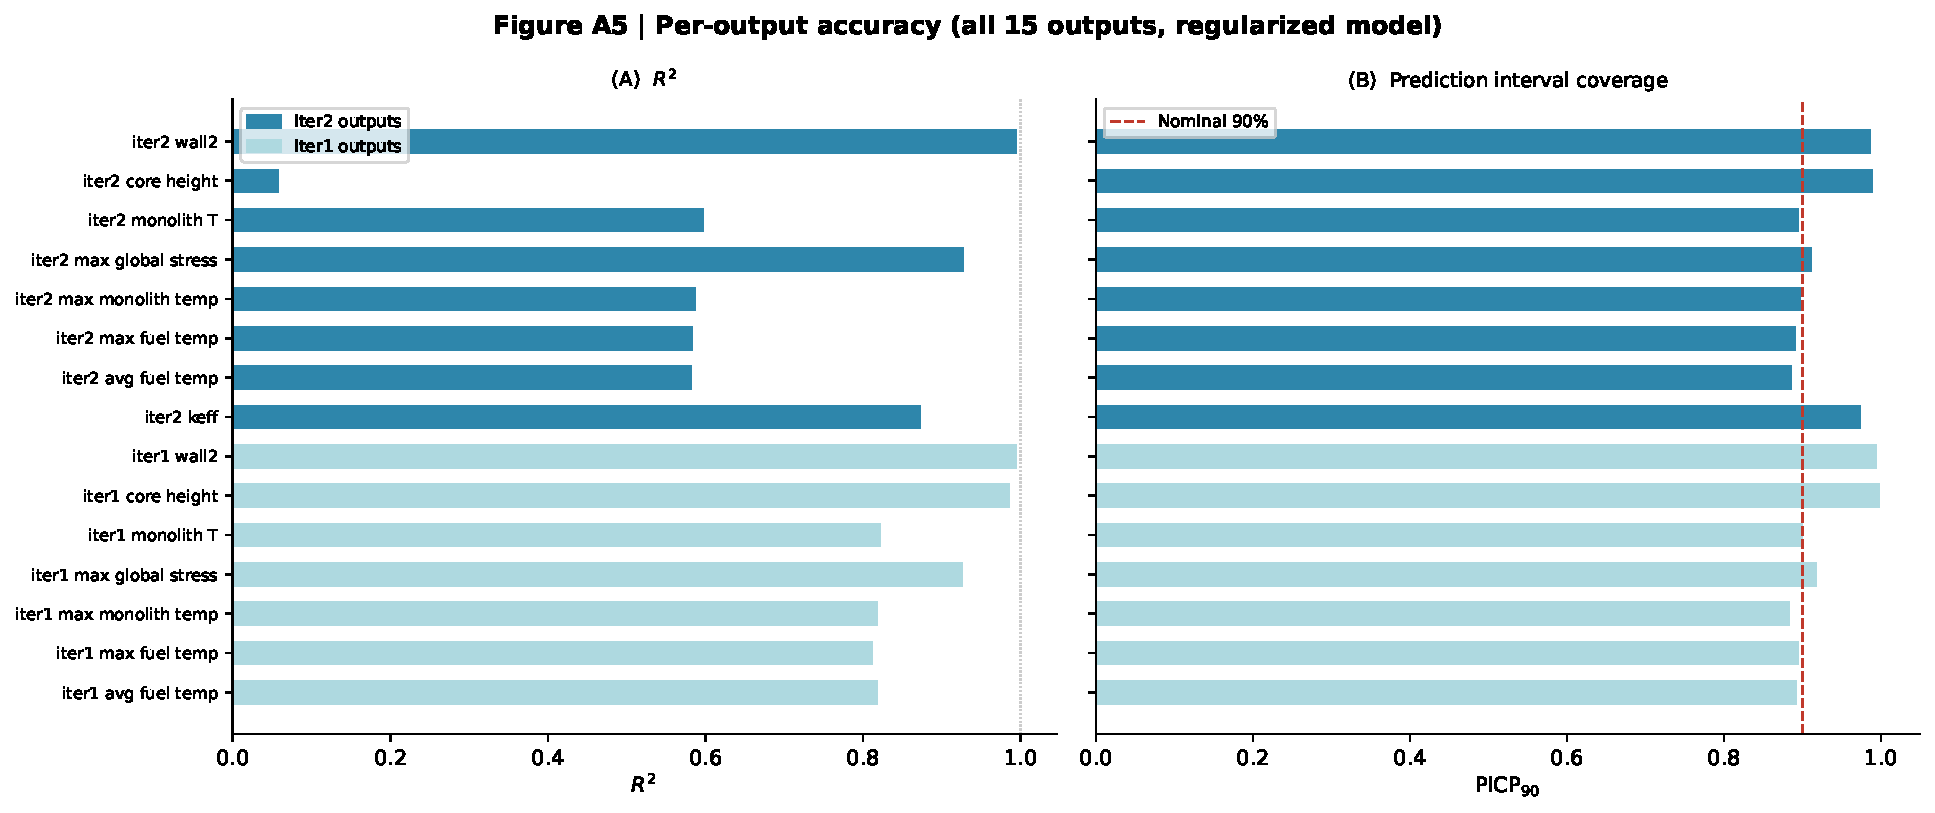
\includegraphics[width=\textwidth]{figA5_per_output_metrics}
  \caption{%
    Per-output accuracy for all 15 physics outputs (Level~2 surrogate, test set).
    (A)~$R^2$; (B)~90\% prediction interval coverage (PICP$_{90}$).
    Blue bars: coupled steady-state outputs; light-blue bars: decoupled (pass~1)
    outputs.
    Wall expansion achieves $R^2=0.996$; coupled temperature outputs show lower
    $R^2\approx0.58$--0.60, reflecting their weaker sensitivity to the 8~material
    inputs in the coupled regime.
    %CN: [可选修改：可改为按输出量物理类型（温度/应力/膨胀）分组排列]
  }\label{fig:per_output}
\end{figure}

% ── Figure A6 ─────────────────────────────────────────────────────────────
%CN: 图A6：4个代表性案例的先验预测分布与后验预测分布对比（应力输出）。
\begin{figure}[ht]
  \centering
  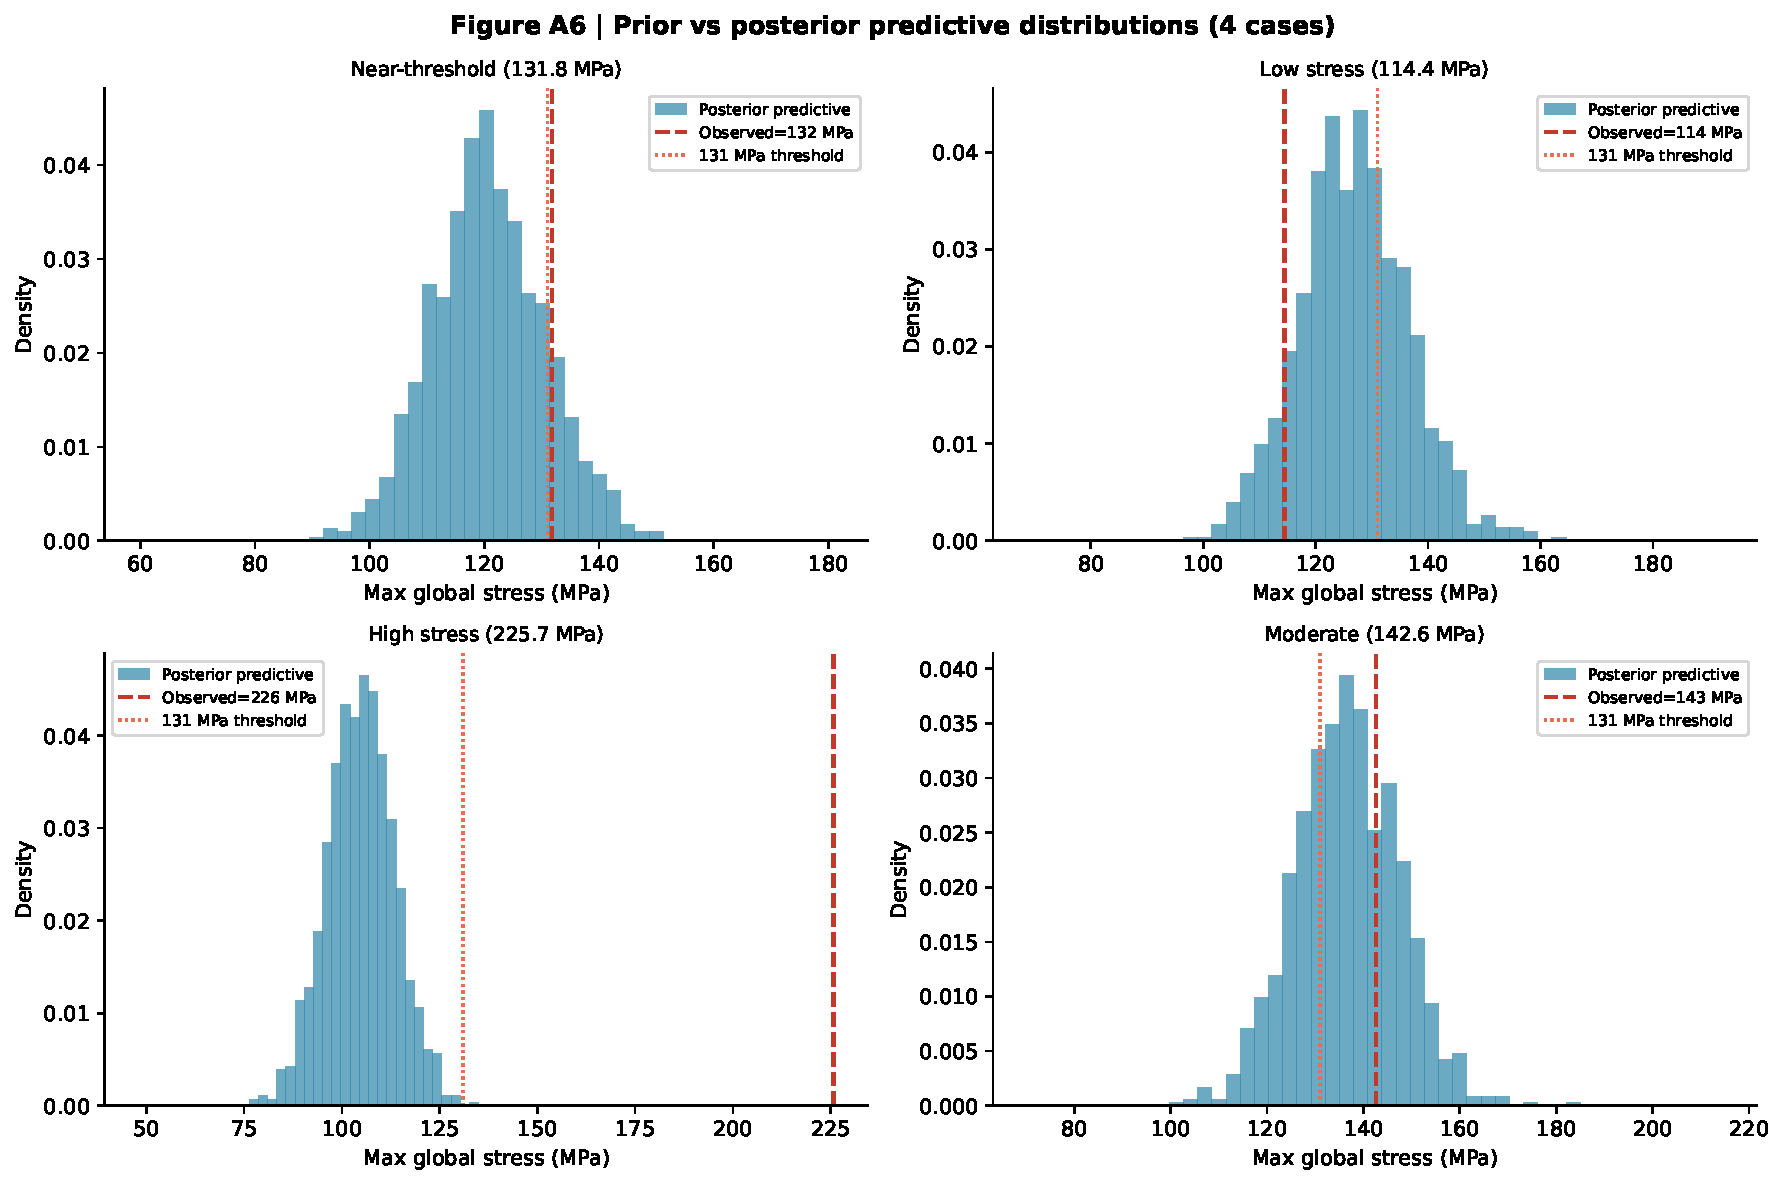
\includegraphics[width=\textwidth]{figA6_prior_post_predictive}
  \caption{%
    Prior predictive (grey) vs.\ posterior predictive (blue) stress distributions
    for four representative benchmark cases (coupled steady-state max global stress).
    The observed stress (red dashed) and design threshold (orange dotted,
    \SI{131}{MPa}) are indicated.
    Posterior updating concentrates probability mass near the observed value in all
    four cases, including the high-stress and extreme-stress scenarios.
    %CN: [可选修改：可增加更多案例或调整案例选择]
  }\label{fig:prior_post_pred}
\end{figure}

% ── Figure A7 ─────────────────────────────────────────────────────────────
%CN: 图A7：HeteroMLP架构示意图，展示8维输入→隐藏层→15维均值输出+15维对数方差输出。
\begin{figure}[ht]
  \centering
  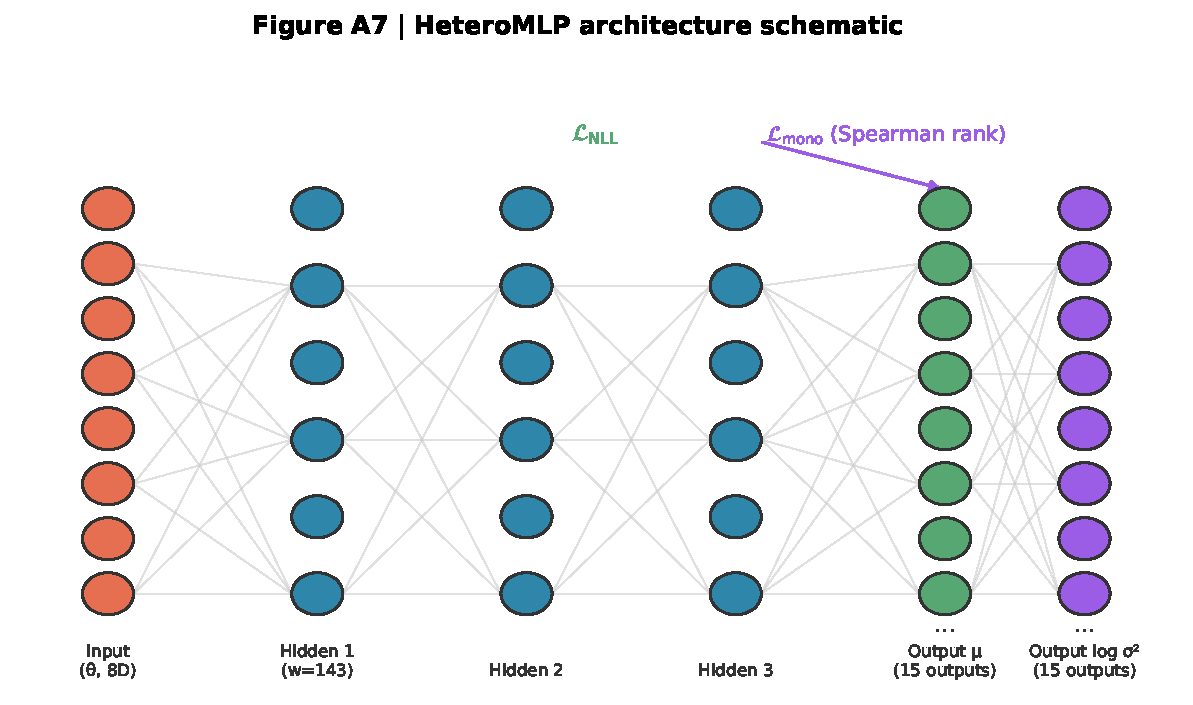
\includegraphics[width=0.85\textwidth]{figA7_bnn_schematic}
  \caption{%
    Schematic of the heteroscedastic multilayer perceptron~(HeteroMLP) architecture.
    The 8-dimensional material parameter vector $\bm{\theta}$ passes through shared
    hidden layers (width 143, depth 3 for Level~2) and is decoded into two heads:
    a~mean output $\bm{\mu}$ and a~log-variance output $\log\bm{\sigma}^2$, each of
    dimension~15.
    The Spearman-rank monotonicity regularization
    $\mathcal{L}_{\mathrm{mono}}$ (Eq.~\ref{eq:mono}) is applied during training
    via the log-variance head.
    %CN: [可选修改：可更新层宽/深度参数，或改为更精确的网络连接图]
  }\label{fig:bnn_schematic}
\end{figure}

% ── Figure A8 ─────────────────────────────────────────────────────────────
%CN: 图A8：训练NLL曲线（训练集和验证集），Level 0（基线）和Level 2（物理正则化）。
%CN: 若训练历史文件缺失则显示占位图。
\begin{figure}[ht]
  \centering
  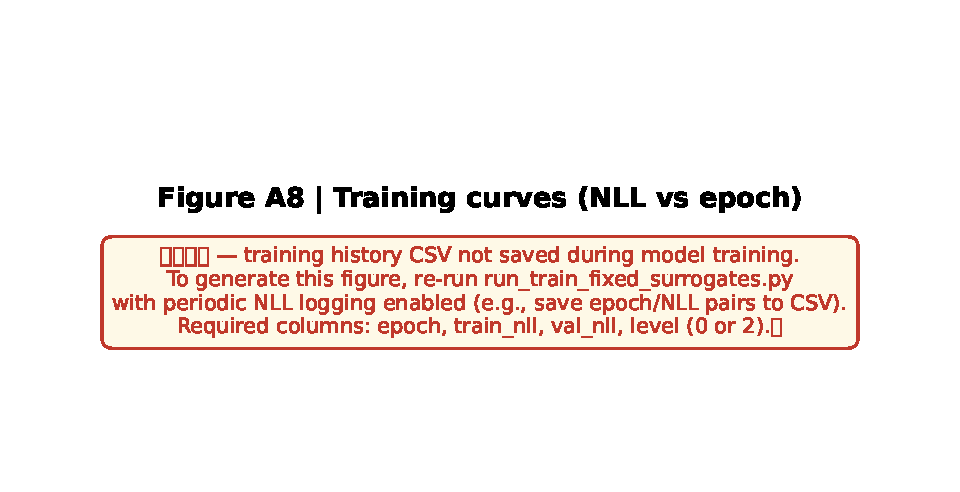
\includegraphics[width=\textwidth]{figA8_training_curves_placeholder}
  \caption{%
    Training curves: negative log-likelihood (NLL) vs.\ epoch for the baseline
    (Level~0) and physics-regularized (Level~2) surrogates.
    (\textit{Placeholder shown; regenerate with actual training history files
    once available by re-running \texttt{run\_train\_fixed\_surrogates.py}.})
    %CN: [待更新：运行训练脚本后替换为实际训练曲线图]
  }\label{fig:training_curves}
\end{figure}

\section{Speedup benchmark details}\label{sec:appendix_speed}

%CN: 附录S7：速度基准详情。
The computational speedup of the Level~2 surrogate versus the coupled HF solver
is summarised in Table~\ref{tab:speed}.

\begin{table}[ht]
\caption{Computational speedup of the surrogate versus the HF solver.}\label{tab:speed}
\begin{tabular}{@{}lrl@{}}
\toprule
Metric & Value & Notes \\
\midrule
Single-sample CPU latency     & \SI{1.55e-4}{s}  & Level~2, CPU \\
Per-sample GPU batch latency  & \SI{1.70e-7}{s}  & Batch size 1024 \\
HF solver (one case)          & \SI{3600}{s}     & OpenMC + FEniCS, 1 CPU node \\
Speedup (single CPU sample)   & $23.2\times10^6$ & \\
Speedup (GPU batch per sample)& $21.2\times10^9$ & \\
\botrule
\end{tabular}
\footnotetext{Source: \texttt{paper\_speedup\_benchmark.json}.}
\end{table}

\end{appendices}

% -----------------------------------------------------------------------
%  References
% -----------------------------------------------------------------------
\bibliography{sn-bibliography}

\end{document}
